\documentclass[12pt]{article}

\usepackage{graphicx}

%math
\usepackage{amsmath}

%%% Figures
\usepackage{caption}      % needed for subfigures
\usepackage{subcaption}   % needed for subfigures

%%% Colors are nice
\usepackage[dvipsnames]{xcolor}   % used for simple color names (e.g. "red")

% own colors
\definecolor{mygreen}{RGB}{28,172,0} % color values Red, Green, Blue
\definecolor{mylilas}{RGB}{170,55,241}

%%% hyperref
\usepackage{hyperref}
\newcommand\myshade{85}
\colorlet{mylinkcolor}{black}
\colorlet{mycitecolor}{black}
\colorlet{myurlcolor}{Aquamarine}
\hypersetup{
  linkcolor  = mylinkcolor!\myshade!black,
  citecolor  = mycitecolor!\myshade!black,
  urlcolor   = myurlcolor!\myshade!black,
  colorlinks = true,
}

% Code
\usepackage{listings}
\lstset{language=Matlab,
    %basicstyle=\color{red},
    breaklines=true,%
    morekeywords={matlab2tikz},
    keywordstyle=\color{blue},%
    morekeywords=[2]{1}, keywordstyle=[2]{\color{black}},
    identifierstyle=\color{black},%
    stringstyle=\color{mylilas},
    commentstyle=\color{mygreen},%
    frame=single,
    showstringspaces=false,%without this there will be a symbol in the places where there is a space
    numbers=left,%
    numberstyle={\tiny \color{black}},% size of the numbers
    numbersep=9pt, % this defines how far the numbers are from the text
    emph=[1]{for,end,break},emphstyle=[1]\color{red}, %some words to emphasise
    emph=[2]{...},emphstyle=[2]\color{mylilas}
    %emph=[2]{word1,word2}, emphstyle=[2]{style},
}

% Clever references need to be loaded after hyperref!
\usepackage[capitalize,nameinlink]{cleveref}       % used for clever references!

%%% Own commands
\newif\ifdebug

\newcommand{\todo}[1]{\ifdebug \textcolor{red}{\textit{\textbf{TODO:}} #1}\else \fi}    % for todos
\newcommand{\info}[1]{\ifdebug \textcolor{blue}{\textit{\textbf{INFO:}} #1}\else \fi}   % for infos
% \newcommand{\cc}[1]{\textcolor{DarkBlue}{\marginnote{\tiny #1}}}     % for comments in the margin

% nicer tables
\usepackage{booktabs}

%tikz party
\usepackage{tikz}
\usetikzlibrary{shapes,arrows}

%supergmiadliche diagrams
\usepackage{smartdiagram}
% set the options
\smartdiagramset{%
  font=\normalsize,
  text width=25mm,
  arrow tip=to,
  uniform arrow color=true,
  arrow color=gray!50!black,
  border color=black,
  set color list={white,white,white}
}

% smaller gaps in enums
\usepackage{enumitem}
\setlist{nosep} % or \setlist{noitemsep} to leave space around whole list


\newtheorem{example}{Example}[section]
\newtheorem{theorem}[example]{Theorem}

\title{Combinatorial Pyramids – Development and Lessons Learned}
\author{David Pfahler}
\date{Technical Report for \\ \emph{Structural Pattern Recognition 2016W}}

%----------------------- Begin of Document -----------------------------------
%-----------------------------------------------------------------------------
\begin{document}

\debugtrue

%-----------------------------------------------------------------------------
%-----------------------------------------------------------------------------
\maketitle

\begin{figure}[!htb]
  \centering
  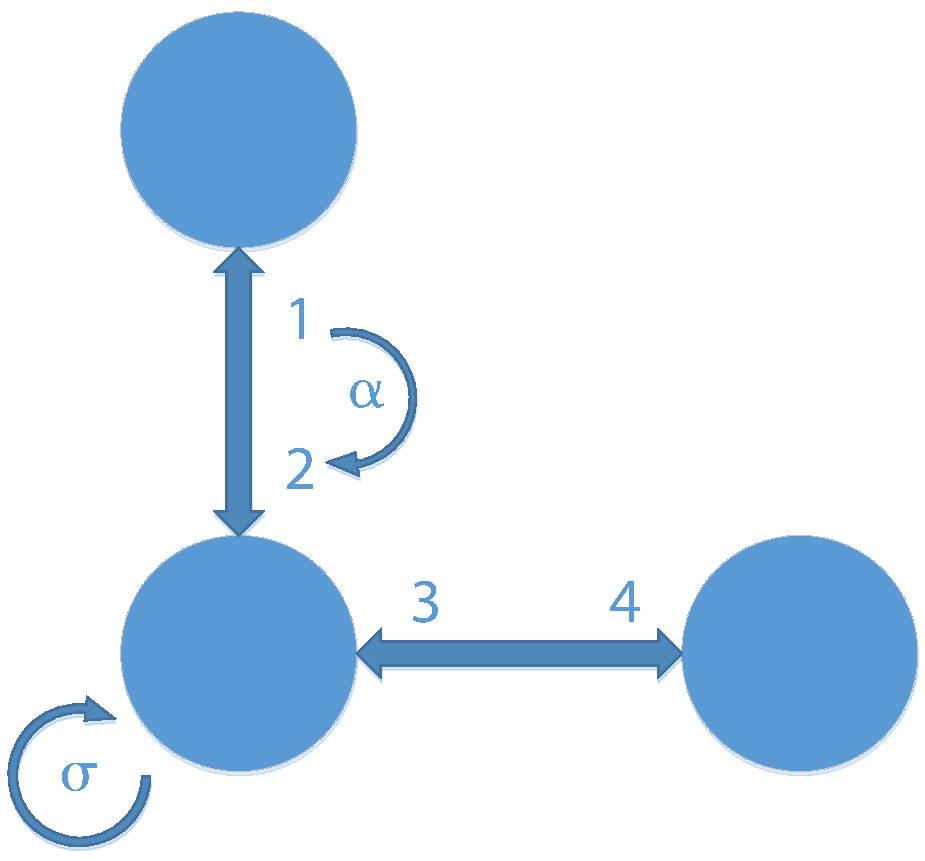
\includegraphics[width=0.3\textwidth]{img/combmap.pdf}
  \caption{A graph with labeled darts. \cref{tab:combmap} shows the involution \( \alpha \) of a dart and the permutation \( \sigma \).}\label{fig:combmap}
\end{figure}

\section{Introduction} % (fold)
\label{sec:introduction}

\subsection{Lecture} % (fold)
\label{sub:lecture}

I wrote this work for the lecture \emph{Structural Pattern Recognition} in the \emph{WS 2016/17}. The content of the lecture was:
\begin{itemize}
  \item Relations between patterns in space and time
  \item Representing structure: strings, arrays, trees, graphs, maps and grammars
  \item Shape and context, embedding in an n-dimensional space
  \item Distances on a given structure graph spectra and eccentricity
  \item Operations on structures and among structures: recognition, parsing
  \item Exact and inexact matching
  \item Modification of structure under motion and tracking
  \item Topology (nD holes, persistence) applications.
\end{itemize}

As my lab exercise in structural pattern recognition I chose the topic ``\emph{Combinatorial Pyramids}'' from the lecture unit 5. To intensify my knowledge from the associated lecture by means of practical examples.

% subsection lecture (end)

\subsection{Problem Specification} % (fold)
\label{sub:problem}

To describe the content of an image it is necessary to extract the objects that an image shows.
The positions of the identified objects to each other gives important information of the context of the image.
An image is most commonly represented by an array of pixels.
To understand the context of the image, it needs to be partitioned into regions.
The context of this regions is called the Region Adjacency Graph (RAG).
\par
To create the RAG the pixel array of the image needs to be transformed into a graph representation.
This is a computational expensive process, because in contrast to the implicit representation in the system memory of a pixel array, a graph representation needs to save pointers for the darts to the nodes (which are the pixels) of the image.
\par
The Combinatorial Map (CM) supports an efficient way to represent the darts in the system memory.
Additionally it enables the application of the graph operations to \emph{contract} and \emph{remove} a dart. \cref{tab:combmap} shows the representation of the CM of \cref{fig:combmap} in the memory.
% subsection problem (end)

\begin{table}[tb]
  \caption{Involution and permutation of the CM from \cref{fig:combmap}}\label{tab:combmap}
  \centering

  \begin{tabular}{lcccc}
  & \textbf{1} & \textbf{2} & \textbf{3} & \textbf{4} \\
  \midrule
     \( \alpha \)& 2 & 1 & 4 & 3\\
     \( \sigma \)& 4 & 2 & 3 & 1\\
  \bottomrule
  \end{tabular}
\end{table}

% section introduction (end)

\section{Development methodology} % (fold)
\label{sec:development_methodology}

I separated the development process into four phases.

\begin{description}
  \item[Phase 1: Existing Work] I did some literature research to get familiar with the topic. (\cref{sub:related_work})
  \item[Phase 2: Meet the Maps] I created an \texttt{Python} application to explore the properties of an neighborhood graph of an image. (\cref{sub:python_implementation})
  \item[Phase 3: Implementation] The actual \texttt{Matlab} implementation is based on the work of the first two phases. (\cref{sec:computation_of_the_dart_values,sec:construction_of_the_initial_cm_level,sec:construction_of_the_pyramid})
  The \cref{fig:cp_creation_process} shows a flowchart of the creation of the CP\@.
  \item[Phase 4: Results] In the end I created some results. (\cref{sec:results})
\end{description}


% Define block styles
\tikzstyle{decision} = [diamond, draw, fill=blue!20,
    text width=4.5em, text badly centered, node distance=3cm, inner sep=0pt]
\tikzstyle{block} = [rectangle, draw, fill=blue!20,
    text width=8em, node distance=3cm, text centered, rounded corners, minimum height=4em]
\tikzstyle{line} = [draw, -latex']
\tikzstyle{cloud} = [draw, ellipse,fill=red!20, node distance=3cm,
    minimum height=2em]
\begin{figure}[tb]
  \centering
  \begin{tikzpicture}[node distance = 2cm, auto]
    % Place nodes
    \node [cloud] (start) {start};
    \node [block,right of=start] (values) {Compute dart values (\cref{sec:computation_of_the_dart_values})};
    \node [block,right of=values, node distance=5cm] (init) {Build initial CM level (\cref{sec:construction_of_the_initial_cm_level})};
    \node [decision,below of=init] (top) {top level reached?};
    \node [block,below of=top,left of=top] (next) {Build Next Level (\cref{sec:construction_of_the_pyramid})};
    \node [cloud,right of=top] (end) {End};

    % Draw edges
    \path [line] (start) -- (values);
    \path [line] (values) -- (init);
    \path [line] (init) -- (top);
    \path [line] (top) -- node [near start] {yes} (end);
    \path [line] (next) |- (top);
    \path [line] (top) |- node {no}(next);
\end{tikzpicture}
  \caption{The CP creation process}
  \label{fig:cp_creation_process}
\end{figure}


\subsection{Related work} % (fold)
\label{sub:related_work}

\begin{figure}[tb]
  \centering

  \begin{subfigure}[b]{0.25\textwidth}
        
\includegraphics[width=\textwidth]{img/prip1}
        \caption{}\label{fig:prip1}
    \end{subfigure}
    ~
    \begin{subfigure}[b]{0.25\textwidth}
        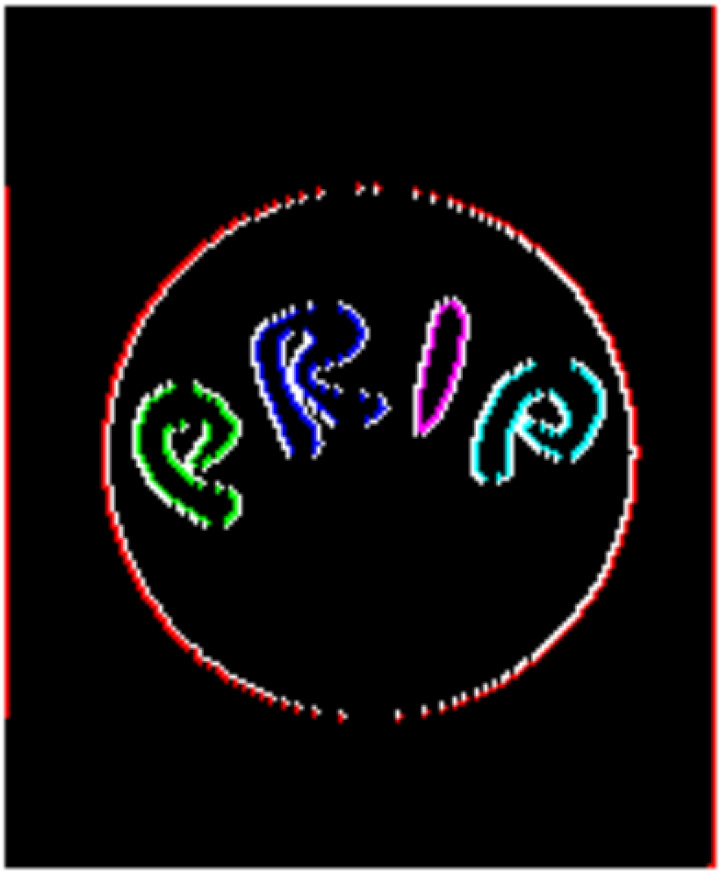
\includegraphics[width=\textwidth]{img/prip2}
        \caption{}\label{fig:prip2}
    \end{subfigure}
    ~
    \begin{subfigure}[b]{0.4\textwidth}
        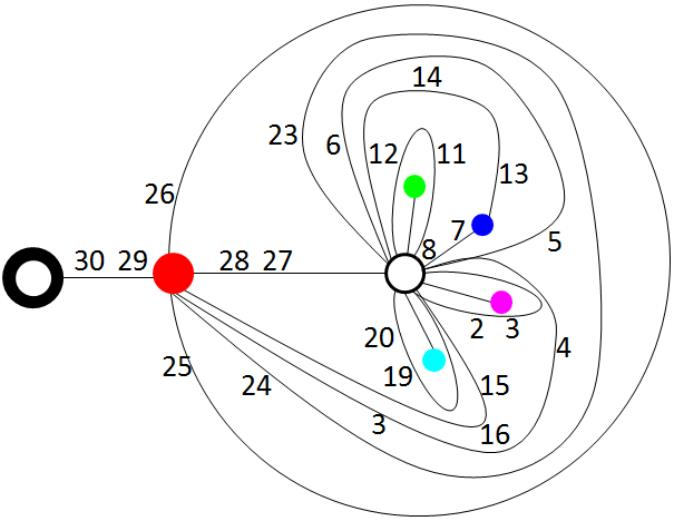
\includegraphics[width=\textwidth]{img/prip3}
        \caption{}\label{fig:prip3}
    \end{subfigure}

    \begin{subfigure}[b]{0.4\textwidth}
        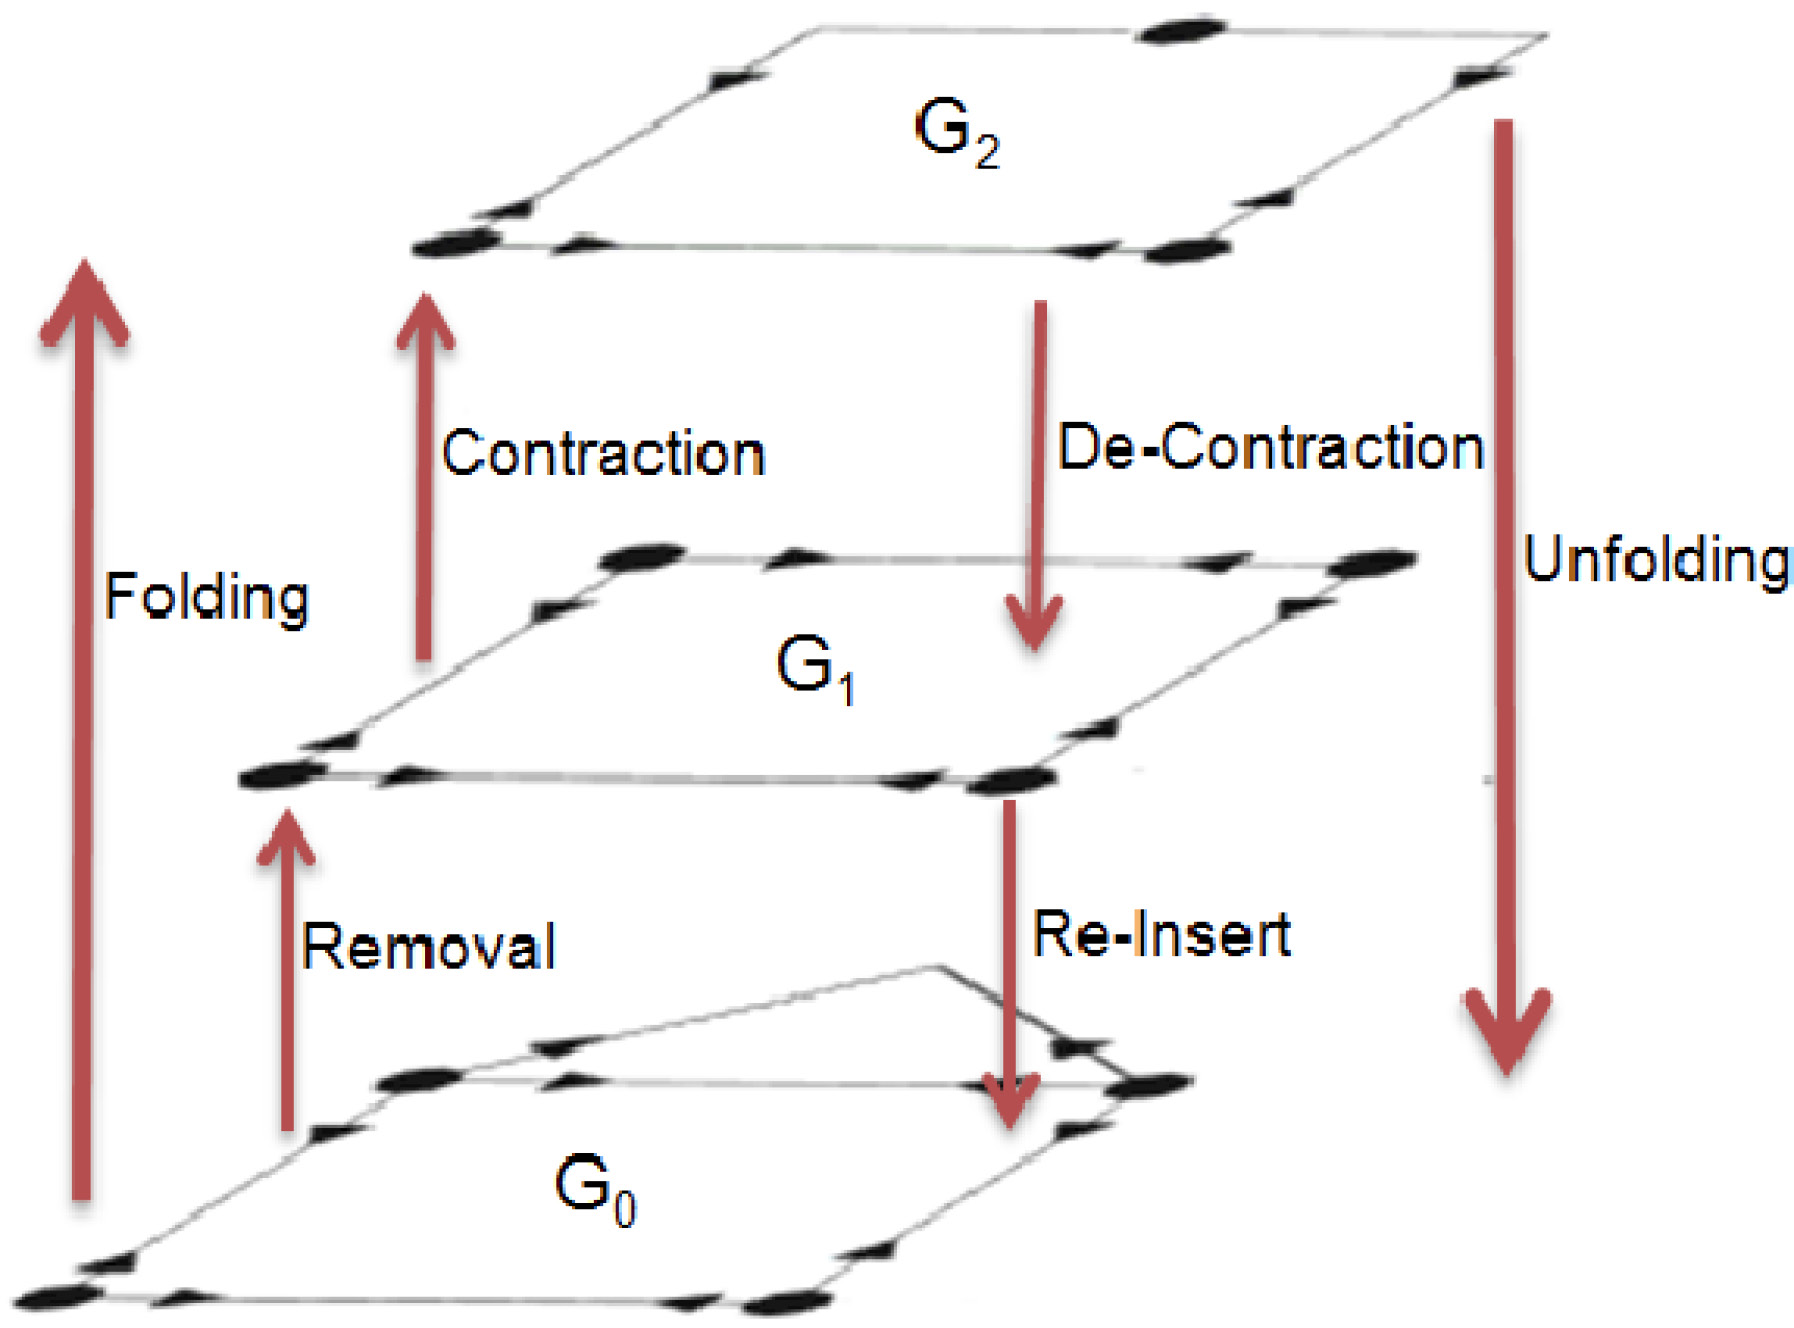
\includegraphics[width=\textwidth]{img/combine_remove.jpg}
        \caption{}\label{fig:combine_remove}
    \end{subfigure}

  \caption{(a) an input image. (b) the segmented image at the first level. (c) the top level of the combinatorial pyramid. (d) Combine and remove operations on a graph}\label{fig:prip}
\end{figure}

The work from Torres and Kropatsch~\cite{torrescanonical} presents a technical report about operations on a CP\@.
The operations I used in my work are the removal of a dart and the contraction of a two darts. These operations are presented in detail later.
\par
\cref{fig:combine_remove} shows the creation of a CP with these two operations on a small graph and also the unfolding of the pyramid with the inverse operations. \cref{fig:prip2} shows all darts that can be contracted or removed from the input image \cref{fig:prip1}. \cref{fig:prip3} shows the top of the CP, which is the RAG of the input image.
\par
The work from Brun and Kropatsch~\cite{brun2001introduction} is an introduction to the CP\@. It presents background information to the contraction
kernel of the CP\@. \cref{fig:creationg_of_a_kernel} shows the creation of a contraction kernel. From the neighborhood graph of the input image (\cref{fig:contract_kernel1}) survivor nodes are selected (\cref{fig:contract_kernel2}). A spanning forest is created, so that every node of the original graph can only be reached from one survivor node (\cref{fig:contract_kernel3}). Then every created tree is contracted into the surviving node and these nodes are connected again (\cref{fig:contract_kernel4}). \cref{fig:contract_kernel5,fig:contract_kernel6,fig:contract_kernel7,fig:contract_kernel8} show the same steps again for this created new pyramid level.
\par

\begin{figure}[tb]
  \centering
  \begin{subfigure}[b]{0.2\textwidth}
      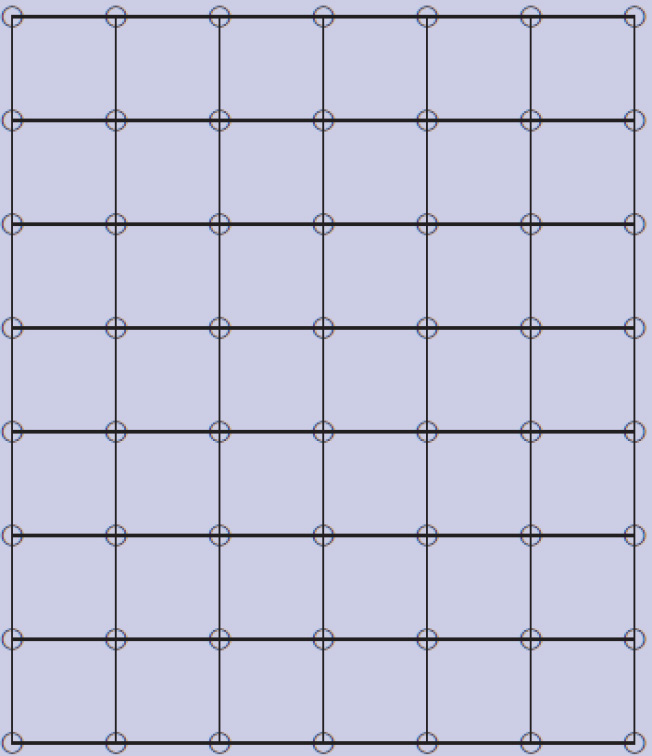
\includegraphics[width=\textwidth]{img/contract_kernel2}
      \caption{}\label{fig:contract_kernel1}
  \end{subfigure}
  ~
  \begin{subfigure}[b]{0.2\textwidth}
      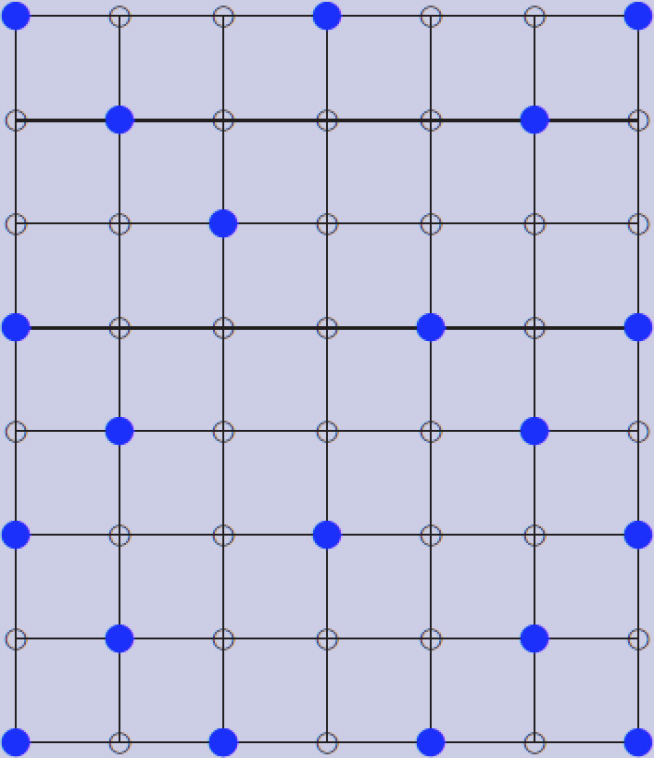
\includegraphics[width=\textwidth]{img/contract_kernel3}
      \caption{}\label{fig:contract_kernel2}
  \end{subfigure}
  ~
  \begin{subfigure}[b]{0.2\textwidth}
      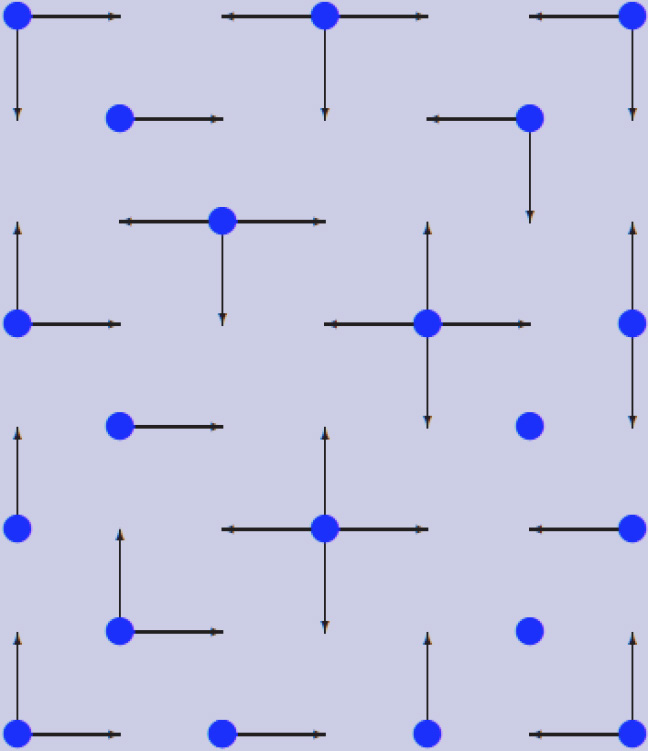
\includegraphics[width=\textwidth]{img/contract_kernel4}
      \caption{}\label{fig:contract_kernel3}
  \end{subfigure}
  ~
  \begin{subfigure}[b]{0.2\textwidth}
      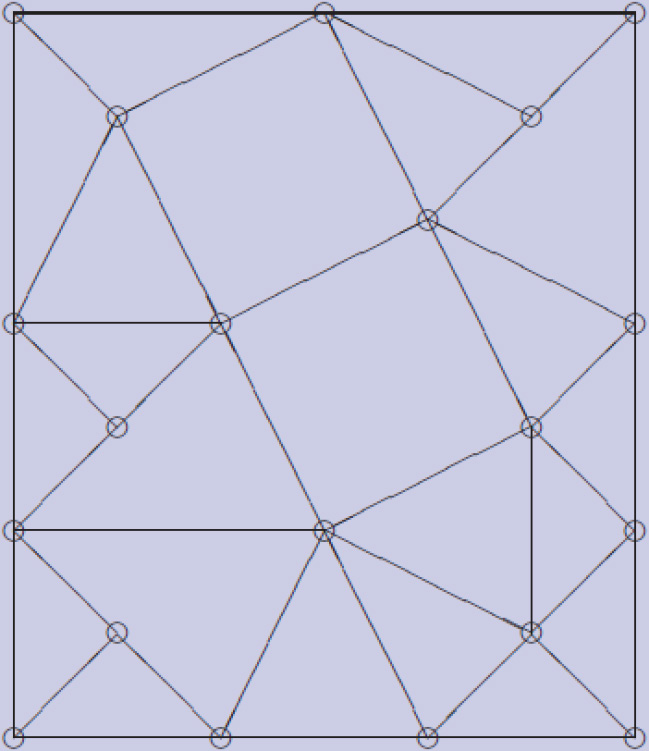
\includegraphics[width=\textwidth]{img/contract_kernel5}
      \caption{}\label{fig:contract_kernel4}
  \end{subfigure}

  \begin{subfigure}[b]{0.2\textwidth}
      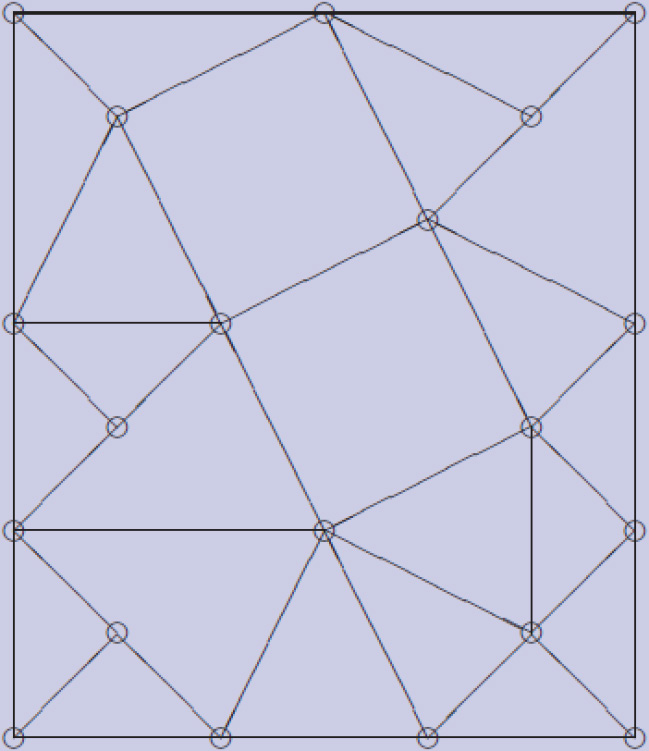
\includegraphics[width=\textwidth]{img/contract_kernel6}
      \caption{}\label{fig:contract_kernel5}
  \end{subfigure}
  ~
  \begin{subfigure}[b]{0.2\textwidth}
      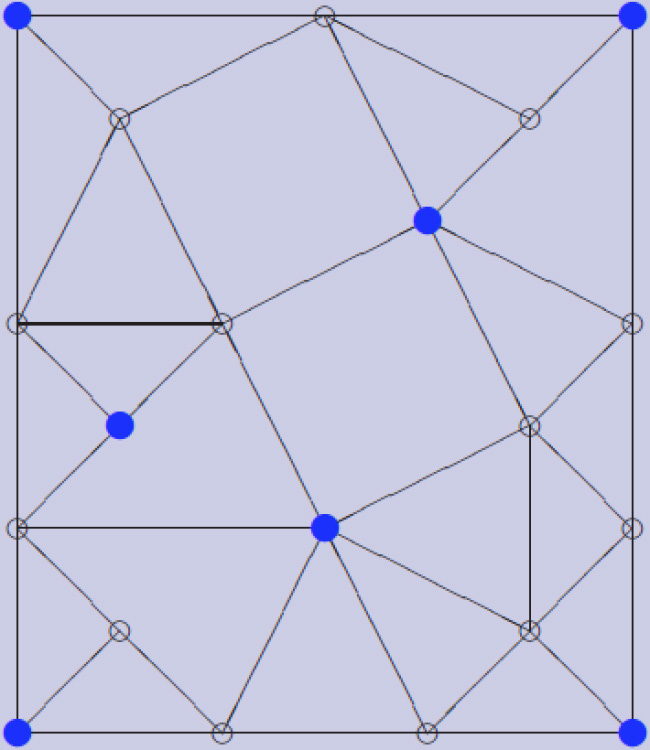
\includegraphics[width=\textwidth]{img/contract_kernel7}
      \caption{}\label{fig:contract_kernel6}
  \end{subfigure}
  ~
  \begin{subfigure}[b]{0.2\textwidth}
      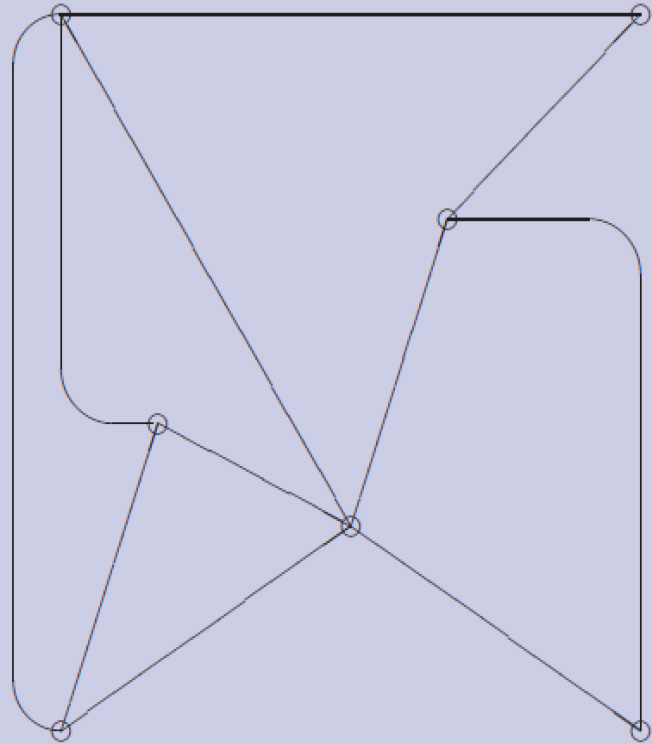
\includegraphics[width=\textwidth]{img/contract_kernel1}
      \caption{}\label{fig:contract_kernel7}
  \end{subfigure}
  ~
  \begin{subfigure}[b]{0.2\textwidth}
      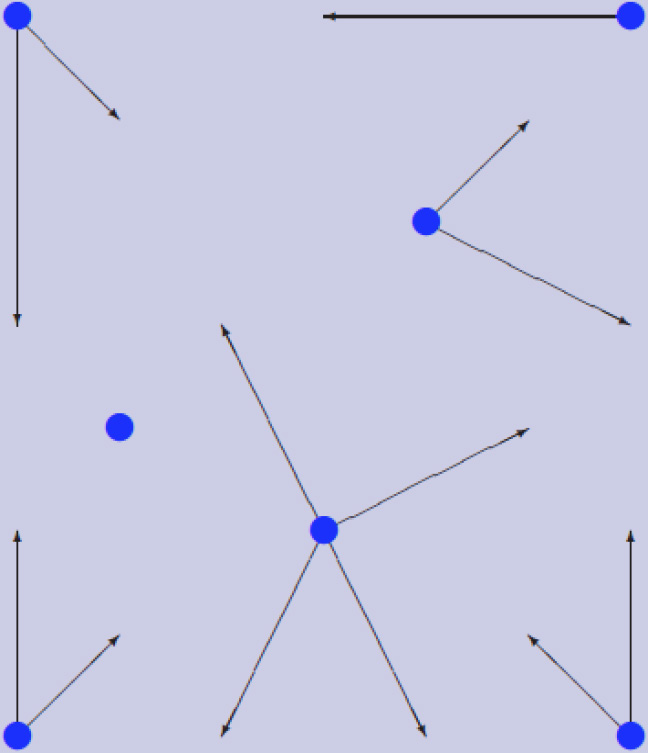
\includegraphics[width=\textwidth]{img/contract_kernel8}
      \caption{}\label{fig:contract_kernel8}
  \end{subfigure}

  \caption{The creation of a contraction kernel}
  \label{fig:creationg_of_a_kernel}
\end{figure}

The further work from Brun and Kropatsch~\cite{brun2003contraction} step into detail of the contraction of darts in parallel. \cref{fig:parallel} shows the conflict of the contraction in parallel. As one can see, if the two marked red darts are selected for contraction and contracted at the same time, it would be undefined were the dart marked with the red question mark would start and end.

\begin{figure}[tb]
  \centering
  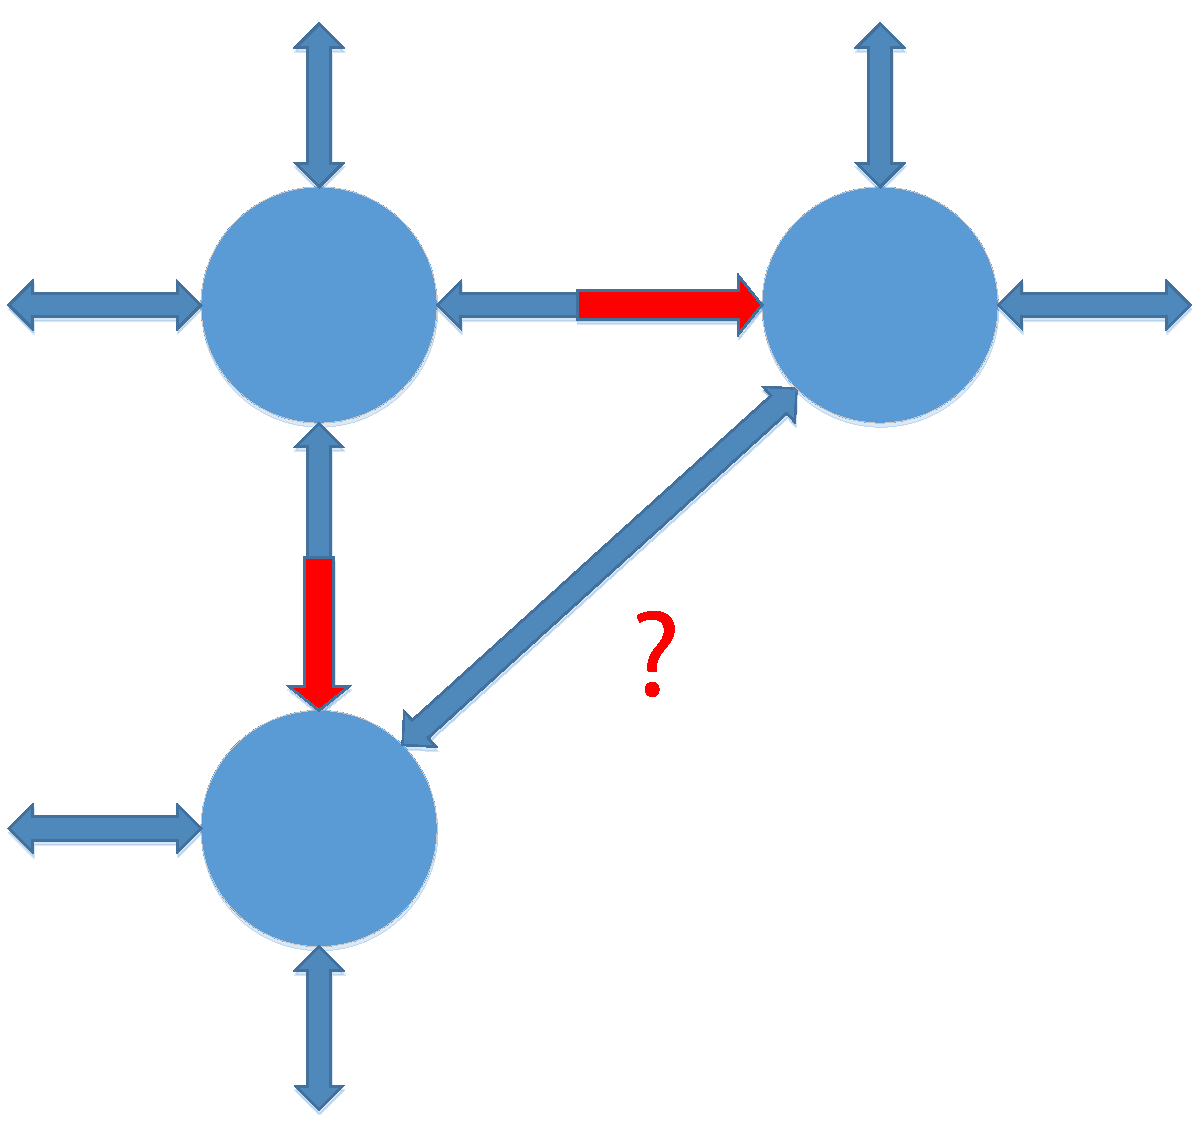
\includegraphics[width=0.4\textwidth]{img/compar.pdf}
  \caption{Contracting in parallel is not trivial}
  \label{fig:parallel}
\end{figure}

% subsection related_work (end)

\subsection{Python implementation} % (fold)
\label{sub:python_implementation}

\begin{lstlisting}[caption={how to use the created \texttt{Python} class},label={lst:python},language=Python]
import CombinatorialMap
map = CombinatorialMap()
map.setSize(3, 5)
map.printNodes()
\end{lstlisting}

To start working with CP I tried to explore the properties of a CM\@. This was not as easy as I thought and there are not many implementations of this matter available. So I decided ti implement a simple \emph{Python} class for CM\@.
This class was not for computations and operations on the CM but for the representation and especially the transformation of an image to a CM\@.
\par
The created class is easy to use as the \cref{lst:python} shows. As already mentioned the class is only a tool to get the representation of an image. In this example the dart indices of a \( 3 \times 5 \) image are shown. The output of this function is shown in \cref{lst:output_python}.

\begin{lstlisting}[caption={The output of the commands of \cref{lst:python}},label={lst:output_python},language=bash,float,floatplacement=H,basicstyle=\scriptsize]
nodes:
    O -  5, 2 -   O -  8, 4 -   O - 11, 7 -   O - 13,10 -   O
    |             |             |             |             |
   1,14          3,17          6,21          9,25         12,29
    |             |             |             |             |
    O - 20,16 -   O - 24,19 -   O - 28,23 -   O - 31,27 -   O
    |             |             |             |             |
  15,32         18,34         22,37         26,40         30,43
    |             |             |             |             |
    O - 36,33 -   O - 39,35 -   O - 42,38 -   O - 44,41 -   O
\end{lstlisting}

Additionally I created functions to receive:
\begin{itemize}
  \item All darts with a specific direction (N, E, S, W)
  \item All involutions of specific darts
  \item Changing the neighborhood function
  \item The orbit of a node
  \item The permutation \( \sigma \) and the involution \( \alpha \) of a set of darts
  \item \ldots
\end{itemize}

% subsection python_implementation (end)

This helped me to understand the dependencies of the indexing of the darts.

% section development_methodology (end)

\section{Computation of the dart values} % (fold)
\label{sec:computation_of_the_dart_values}

A dart in an image is a transition from one pixel to another. In my implementation I used the 4 neighborhood of the pixel for the creation of the image graph.
The value of a transition should represent the change of the pixel value.
So I computed from every pixel the change of the pixel value to every neighbor of their neighborhood (N,E,S,W).
\par
\cref{fig:dart_values} visualizes the resulting dart values for every cardinal direction.

\begin{figure}[tb]
  \centering

  \begin{subfigure}[b]{0.46\textwidth}
        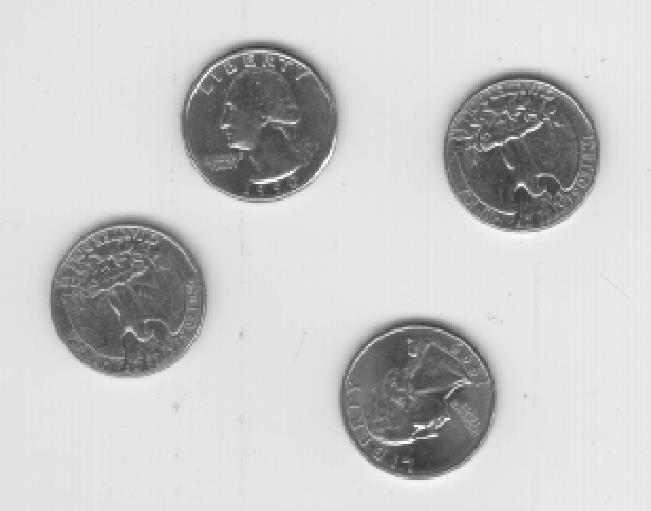
\includegraphics[width=\textwidth]{img/values_init.jpg}
        \caption{}\label{fig:dart_values_init}
    \end{subfigure}
    ~
    \begin{subfigure}[b]{0.45\textwidth}
        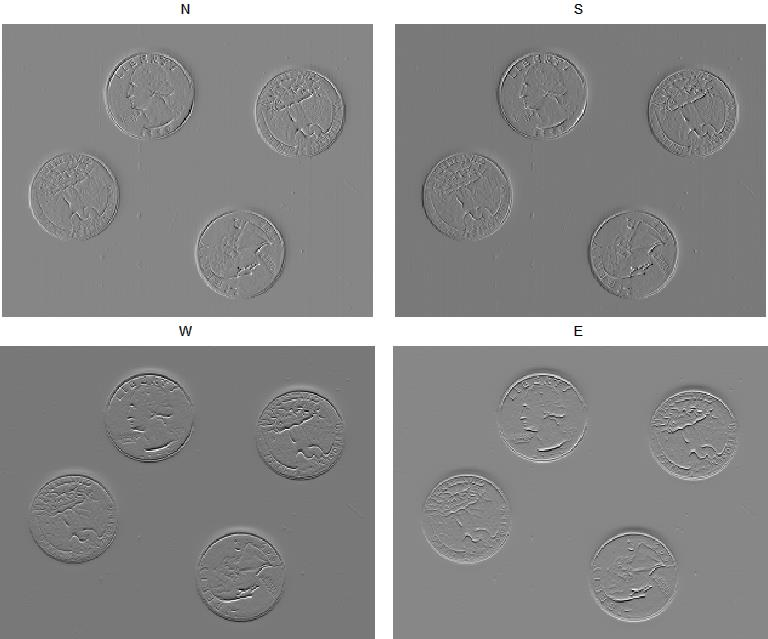
\includegraphics[width=\textwidth]{img/values_new.jpg}
        \caption{}\label{fig:dart_values_news}
    \end{subfigure}

  \caption{(a) The gray scale input image (b) the transition values from every pixel to its North, South, West and East pixel neighbor. The displayed pixel value range of the differences is mapped from [-128,128] to [0,255]}\label{fig:dart_values}
\end{figure}

% section computation_of_the_dart_values (end)

\section{Construction of the initial CM level} % (fold)
\label{sec:construction_of_the_initial_cm_level}

I used the \texttt{Python} implementation presented in \cref{sub:python_implementation} to understand the indexing of the darts.
The following properties of the image need to get calculated to obtain an initial CM\@:
\begin{itemize}
  \item The dart indices \( x \) of the dart values from the previous section.
  \item The permutation \( \sigma(x) \)
  \item The involution \( \alpha(x) \)
  \item The previous dart of the dart index \( \rho(x) := \sigma^{-1}(x)  \)
\end{itemize}

\subsection{Computation of the dart indices} % (fold)
\label{sub:computation_of_the_dart_indices}

The indexing of the dart values is motivated by the output from \cref{lst:output_python}. As one can see the next index with the same direction is gained by adding 4, if it is inside the image.
On the border it is only added by 3, because one dart is missing. Additional similar exceptions occur on the corners.

% subsection computation_of_the_dart_indices (end)

\subsection{Computation of the next index} % (fold)
\label{sub:computation_of_the_next_index}

\begin{table}[tb]
  \caption{The permutation \( \sigma \) of a \( 3 \times 3 \) image}
  \label{tab:permutation}
  \centering

  \tiny
  \begin{tabular}{lrrrrrrrrrrrrrrrrrrrrrrrr}
  \toprule
  \( x \)& 1 & 2 & 3 & 4 & 5 & 6 & 7 & 8 & 9 & 10 & 11 & 12 & 13 & 14 & 15 & 16 & 17 & 18 & 19 & 20 & 21 & 22 & 23 & 24 \\
\( \sigma \)& 2 & 1 & 5 & 3 & 4 & 7 & 6 & 10& 8 & 9 & 13& 14& 12& 11& 16& 17& 15& 19& 18& 21& 22& 20& 24& 23 \\
\( x - \sigma \)& 1 & -1 & 2 & -1 & -1 & 1 & -1 &  2 & -1 & -1 &  2 &  2 &  -1 &  -3 &  1 &  1 &  -2 &  1 &  -1 &  1 &  1 &  -2 &  1 & -1\\
  \bottomrule
  \end{tabular}
\end{table}

By looking at the permutation of an image a pattern can be observed. \cref{tab:permutation} shows the permutation \( \sigma \) of a \( 3 \times 3 \) image. One can see that for one row within the image the next dart has an image difference of:
\begin{lstlisting}
repmat([2; 2; -1; -3], width-2, 1)
\end{lstlisting}
Which results in the differences for the whole middle of the image:

\begin{lstlisting}
repmat( ...
  [next_darts_one_row; 1; 1; -2; 2; -1; -1], ...
  height-2, 1)
\end{lstlisting}

Once again special cases occur for the borders of the image.

% subsection computation_of_the_next_index (end)

\subsection{Computation of the other properties} % (fold)
\label{sub:computation_of_the_other_properties}

The other properties of the image are more easy to calculate:

\begin{itemize}
  \item The involution \( \alpha \) for the indices of the darts that point to the north are the indices that point to south (and vice versa).
  \item The previous dart \( \rho \)  of the next dart \( \sigma \) is the dart \( x \) itself.
\end{itemize}

\begin{lstlisting}
cm.involution(N) = S
cm.involution(S) = N
cm.involution(E) = W
cm.involution(W) = E

cm.prev(cm.next) = 1:num_darts
\end{lstlisting}


% subsection computation_of_the_other_properties (end)

% section construction_of_the_initial_cm_level (end)

\section{Construction of the pyramid} % (fold)
\label{sec:construction_of_the_pyramid}

\begin{figure}[tb]
\centering
\smartdiagram[circular diagram:clockwise]
{
  Compute Contraction Kernel (\cref{sub:compute_the_contraction_kernel}),
  Contract Darts (\cref{sub:contraction}),
  Simplify Level (\cref{sub:simplification})
}
\caption{The creation loop of the pyramid}%
\label{fig:creation loop}
\end{figure}

After the initial CM is created the map needs to be reduced. The iterative reduction of the CM with the loop described in \cref{fig:creation loop} the CP is created.

\subsection{Compute the contraction kernel} % (fold)
\label{sub:compute_the_contraction_kernel}

\begin{figure}[tb]
  \centering
  \vspace{-10 mm}

  \begin{subfigure}[b]{0.15\textwidth}
      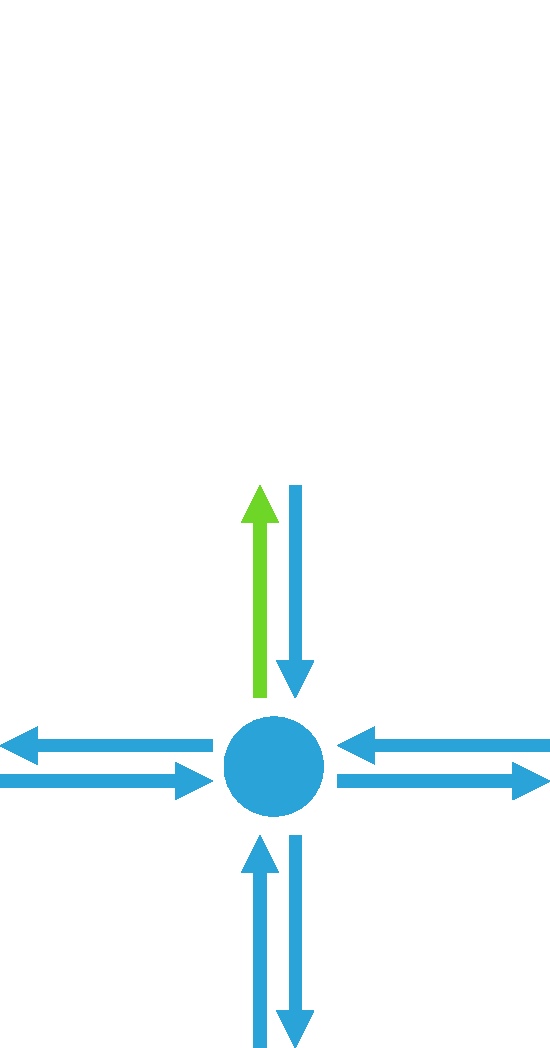
\includegraphics[width=\textwidth]{img/1}
      \caption{}\label{fig:contraction_kernel_greedy1}
  \end{subfigure}
  ~
  \begin{subfigure}[b]{0.15\textwidth}
      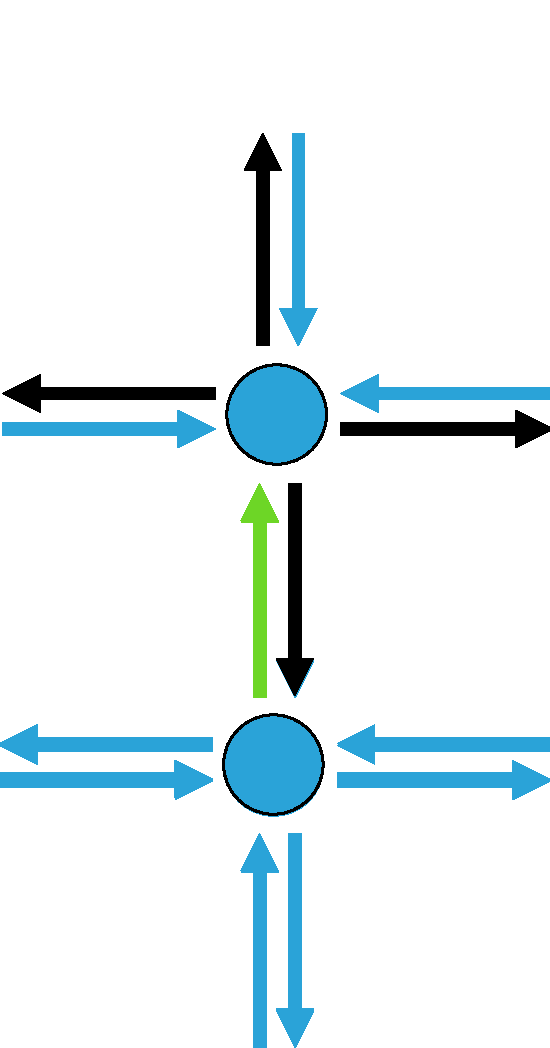
\includegraphics[width=\textwidth]{img/2}
      \caption{}\label{fig:contraction_kernel_greedy2}
  \end{subfigure}
  ~
  \begin{subfigure}[b]{0.15\textwidth}
      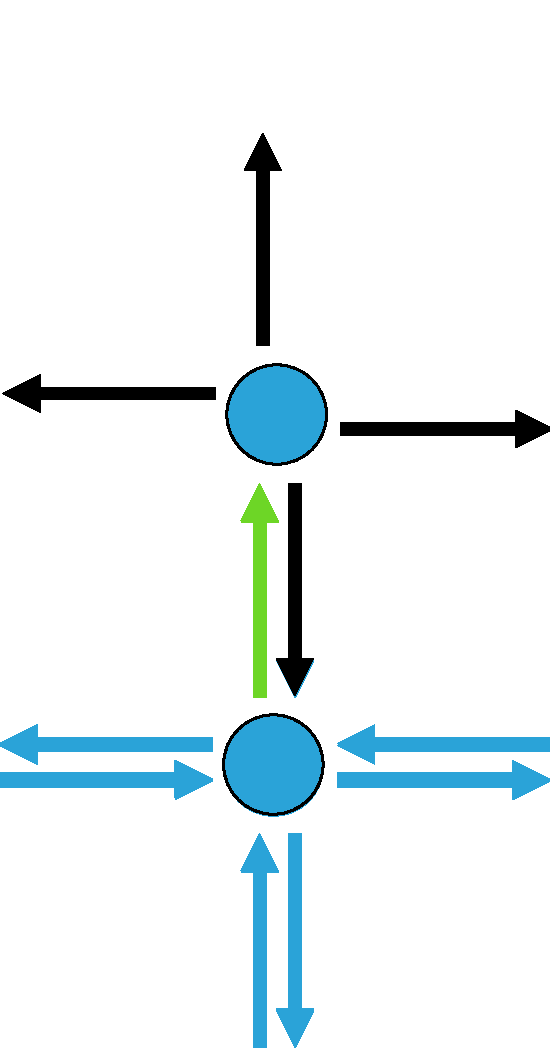
\includegraphics[width=\textwidth]{img/3}
      \caption{}\label{fig:contraction_kernel_greedy3}
  \end{subfigure}
  ~
  \begin{subfigure}[b]{0.15\textwidth}
      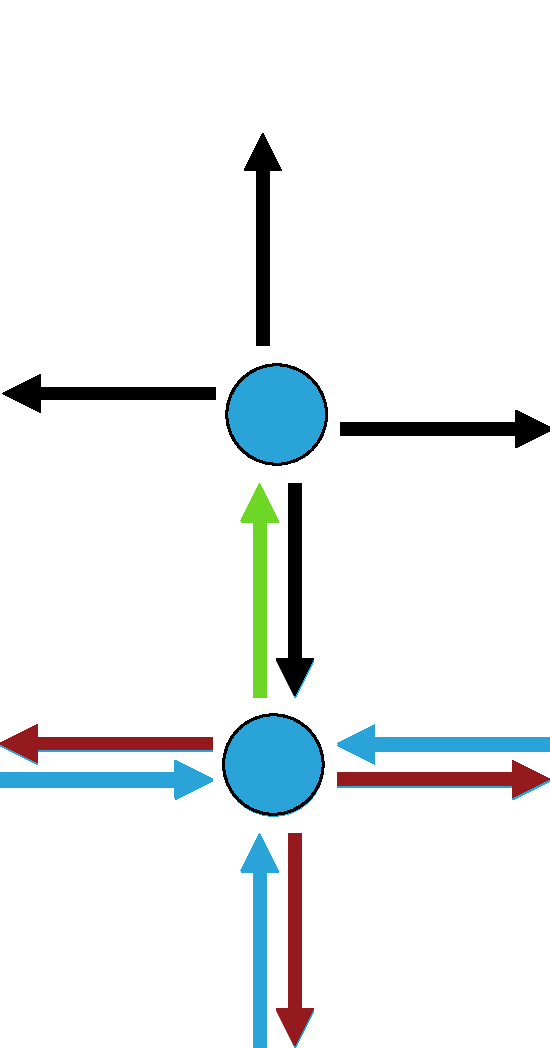
\includegraphics[width=\textwidth]{img/4}
      \caption{}\label{fig:contraction_kernel_greedy4}
  \end{subfigure}
  ~
  \begin{subfigure}[b]{0.15\textwidth}
      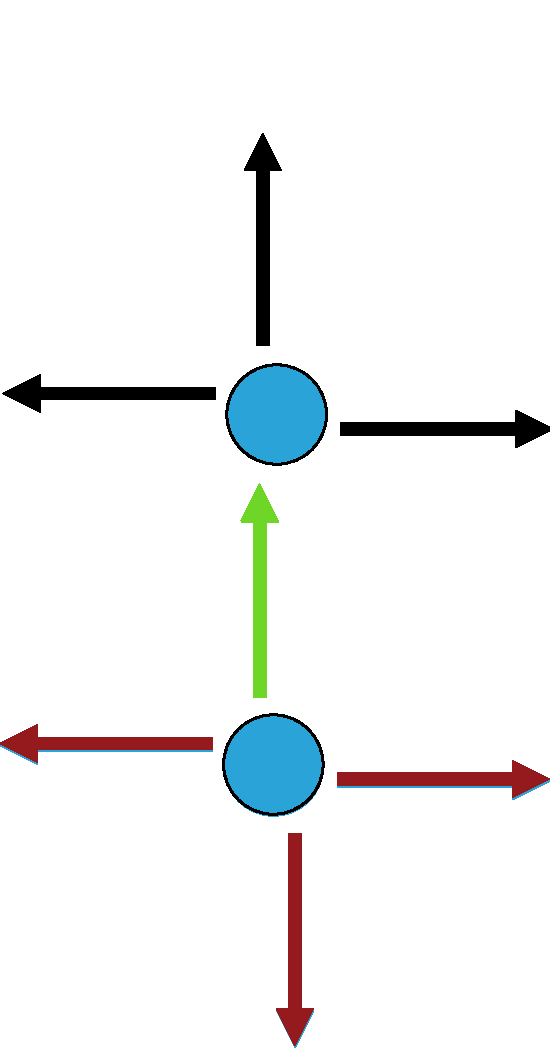
\includegraphics[width=\textwidth]{img/5}
      \caption{}\label{fig:contraction_kernel_greedy5}
  \end{subfigure}

  \caption{(a) Assign next best dart for the contraction kernel (b) Get the involution of the dart and the orbit of the involution (c) now remove the involution of the involution orbit from the set of valid darts (d) now get the orbit of the dart (e) And remove its involution}
  \label{fig:contraction_kernel_greedy}
\end{figure}

Initially the darts are sorted by its values. This sorting only needs to be done once for the initial CM\@. For the reduction a contraction kernel needs to be defined (\cref{sub:related_work}). I implemented a greedy algorithm to calculate the kernel.
\par
\cref{fig:contraction_kernel_greedy} shows the creation of the kernel.
\begin{itemize}
  \item First assign next best dart for the contraction kernel (\cref{fig:contraction_kernel_greedy1})
  \item Then get the involution of the dart and the orbit of the involution (\cref{fig:contraction_kernel_greedy2})
  \item Now remove the involution of the involution orbit from the set of valid darts (\cref{fig:contraction_kernel_greedy3})
  \item Now get the orbit of the dart (\cref{fig:contraction_kernel_greedy4})
  \item And remove its involution
  \item Repeat until there are no valid darts left
\end{itemize}

There are two exceptions for the adding of darts to the contraction kernel:
\emph{Self loops} and \emph{pending edges}.
\par
A self loop is detected by checking if the orbit of the dart is the same as the orbit of the involution of the dart. And the orbit of a pending edge contains only the edge itself.

The red darts in \cref{fig:dart_contract} show the contraction kernels for three different images.

\begin{figure}[tb]
  \centering
    \begin{subfigure}[t]{0.3\textwidth}
      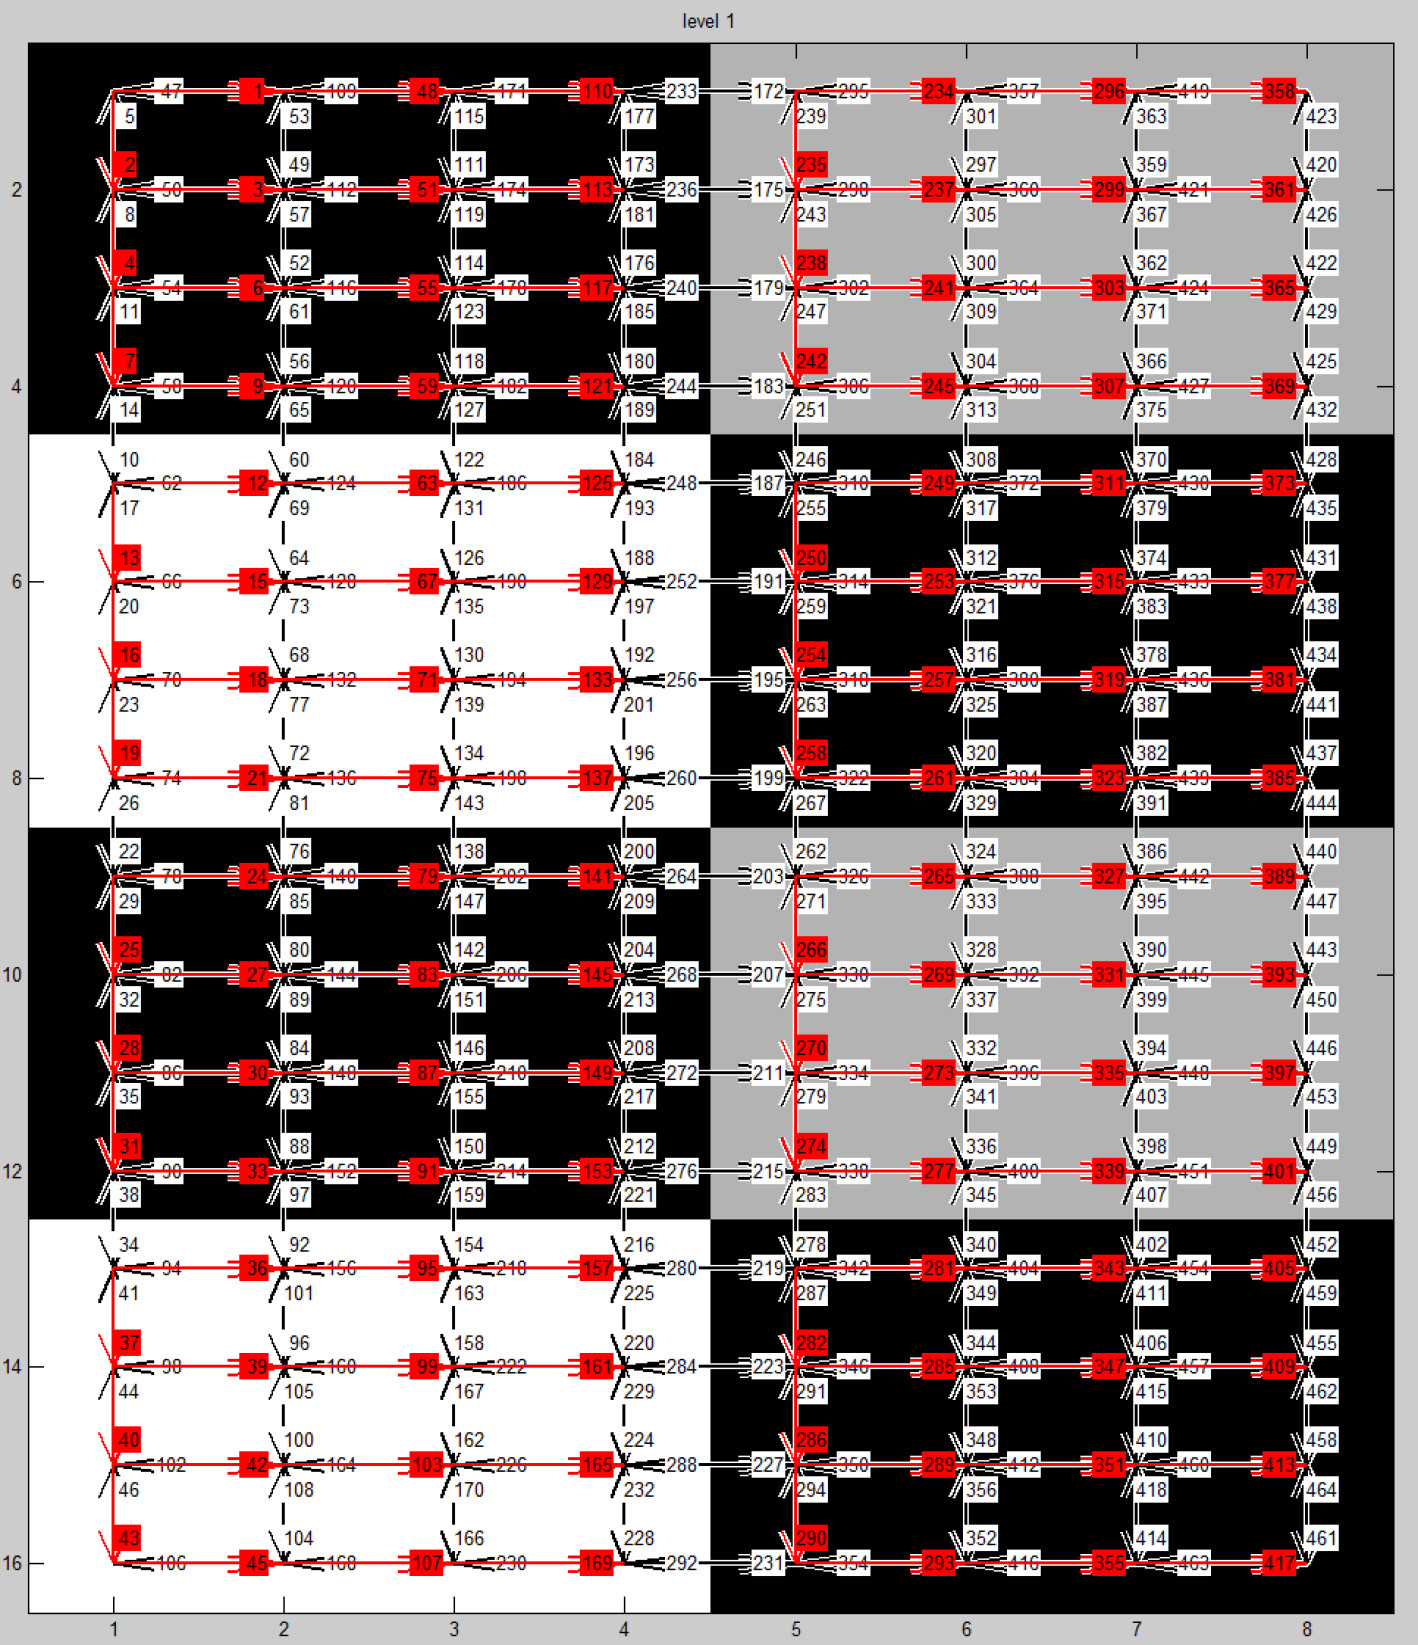
\includegraphics[width=\textwidth]{img/contract2.jpg}
      \caption{}\label{fig:dart_contract2}
    \end{subfigure}
    ~
    \begin{subfigure}[t]{0.3\textwidth}
      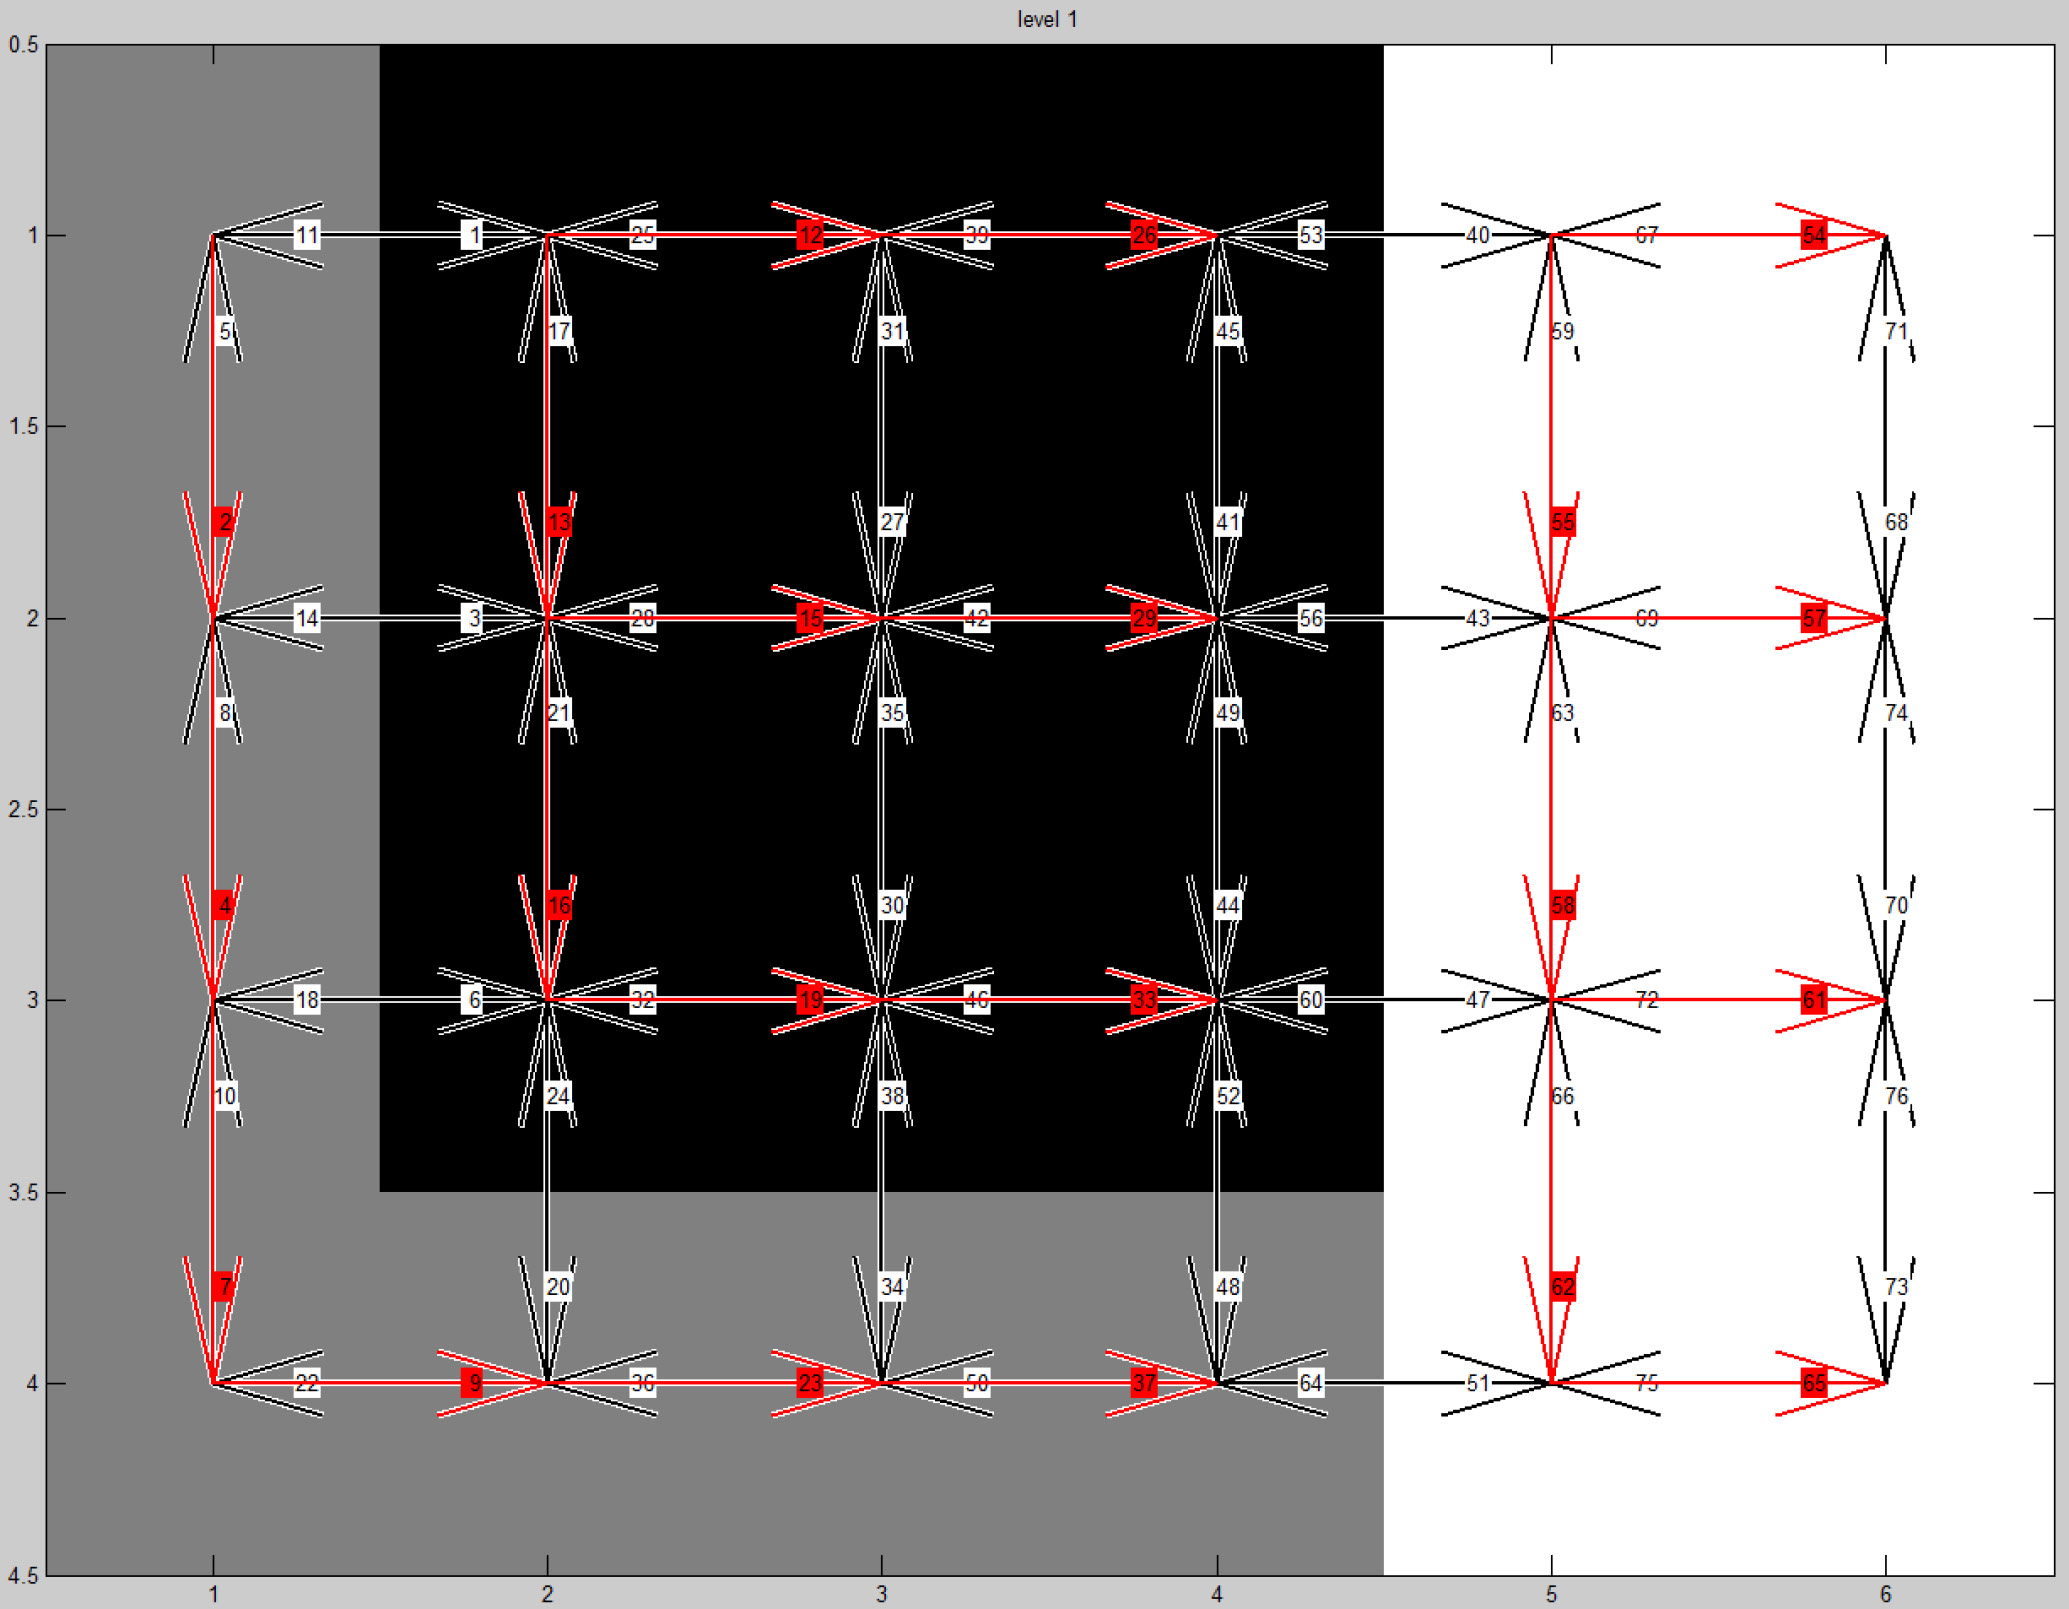
\includegraphics[width=\textwidth]{img/contract3.jpg}
      \caption{}\label{fig:dart_contract3}
    \end{subfigure}
    ~
    \begin{subfigure}[t]{0.3\textwidth}
      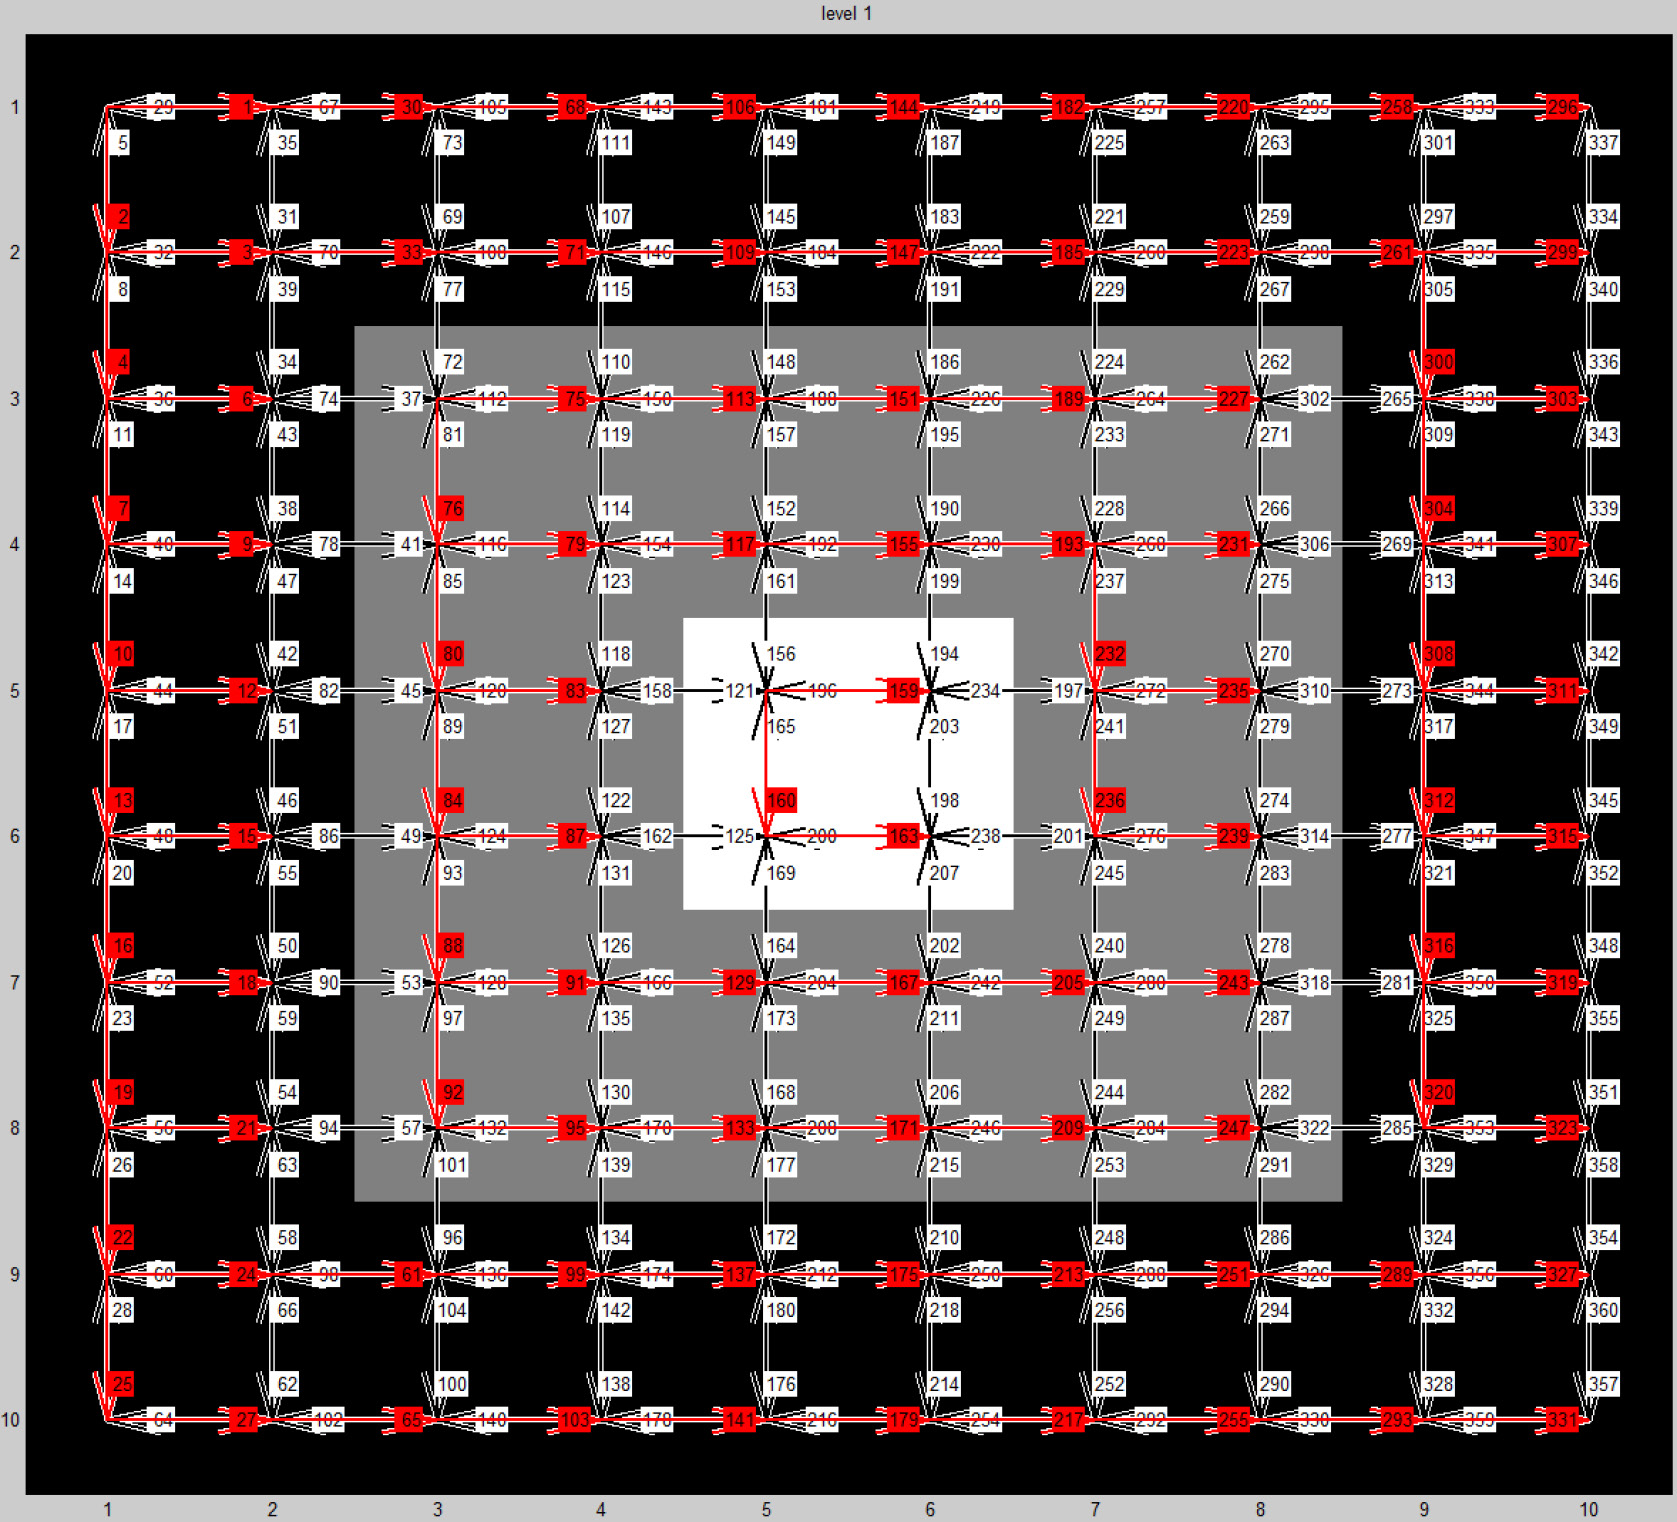
\includegraphics[width=\textwidth]{img/contract1.jpg}
      \caption{}\label{fig:dart_contract1}
    \end{subfigure}
  \caption{The red darts show the contraction kernels for the three images.}\label{fig:dart_contract}
\end{figure}

% subsection compute_the_contraction_kernel (end)

\subsection{Contraction} % (fold)
\label{sub:contraction}

The contraction of a dart in a CM is calculated with only 4 changes of the CM\@. The next \( \sigma'(\rho(x))\) and previous \( \rho'(\sigma(x))\) dart need to get updated for the dart  \( x \) and its involution \( \alpha(x) \). And  \( x \) and \( \alpha(x) \) are removed from the set of active darts.

\begin{align}
  \sigma'(\rho(x))   &:= \sigma(\alpha(x))    \\
  \sigma'(\rho(\alpha(x)))  &:= \sigma(x)     \\
  \rho'(\sigma(x))   &:= \rho(\alpha(x))      \\
  \rho'(\sigma(\alpha(x)))  &:= \rho(x)
\end{align}

% subsection contraction (end)

\subsection{Simplification} % (fold)
\label{sub:simplification}

\begin{figure}[tb]
  \centering
  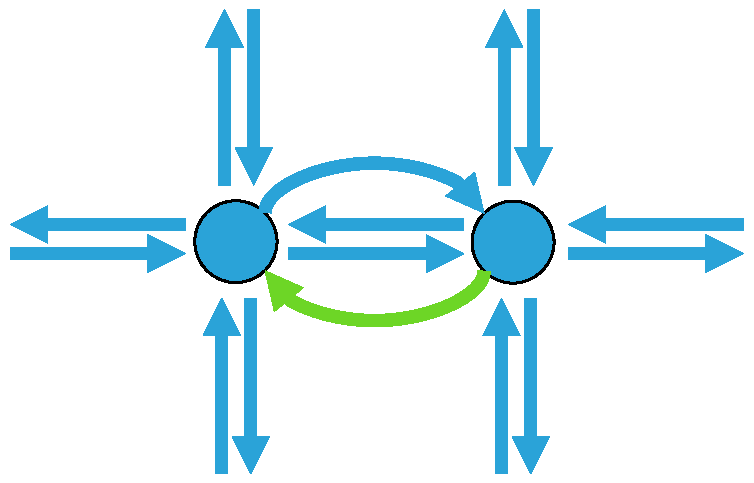
\includegraphics[width=0.6\textwidth]{img/face.pdf}
  \caption{The number of darts of this face is less than 2 and it can be removed}
  \label{fig:faces}
\end{figure}

When contracting darts double edges and self-direct-loops are created. By removing these darts the pyramid is easier to read.

For detecting them the face of a dart \(x\) is needed:

\begin{itemize}
  \item Get the involution \(\alpha(x)\)
  \item Get the previous of the involution of the dart \(\rho(\alpha(x))\)
  \item add this to the face and repeat for this dart until the initial dart is reached
\end{itemize}

If the number of darts in the face is smaller than 3 the dart can be removed.
\cref{fig:faces} shows a configuration of darts that build up a double edge. The face of the green marked dart has two darts, which can be removed.
The removal operation is similar to the contract operation:

\begin{align}
  \sigma'(\rho(x))   &:= \sigma(x)                \\
  \sigma'(\rho(\alpha(x)))  &:= \sigma(\alpha(x)) \\
  \rho'(\sigma(x))   &:= \rho(x)                  \\
  \rho'(\sigma(\alpha(x)))  &:= \rho(\alpha(x))
\end{align}

If \( x \) is equal to \( \alpha(x) \) a self-direct-loop is detected. The removal of this has to be treated differently:

\begin{align}
  \sigma'(\rho(x))  &:= \sigma(\alpha(x)) \\
\end{align}

\cref{fig:dart_simply} shows the simplification after the contraction of the contraction kernel. As one can see the number of darts is reduced significantly.

\begin{figure}[tb]
  \centering

    \begin{subfigure}[b]{0.3\textwidth}
      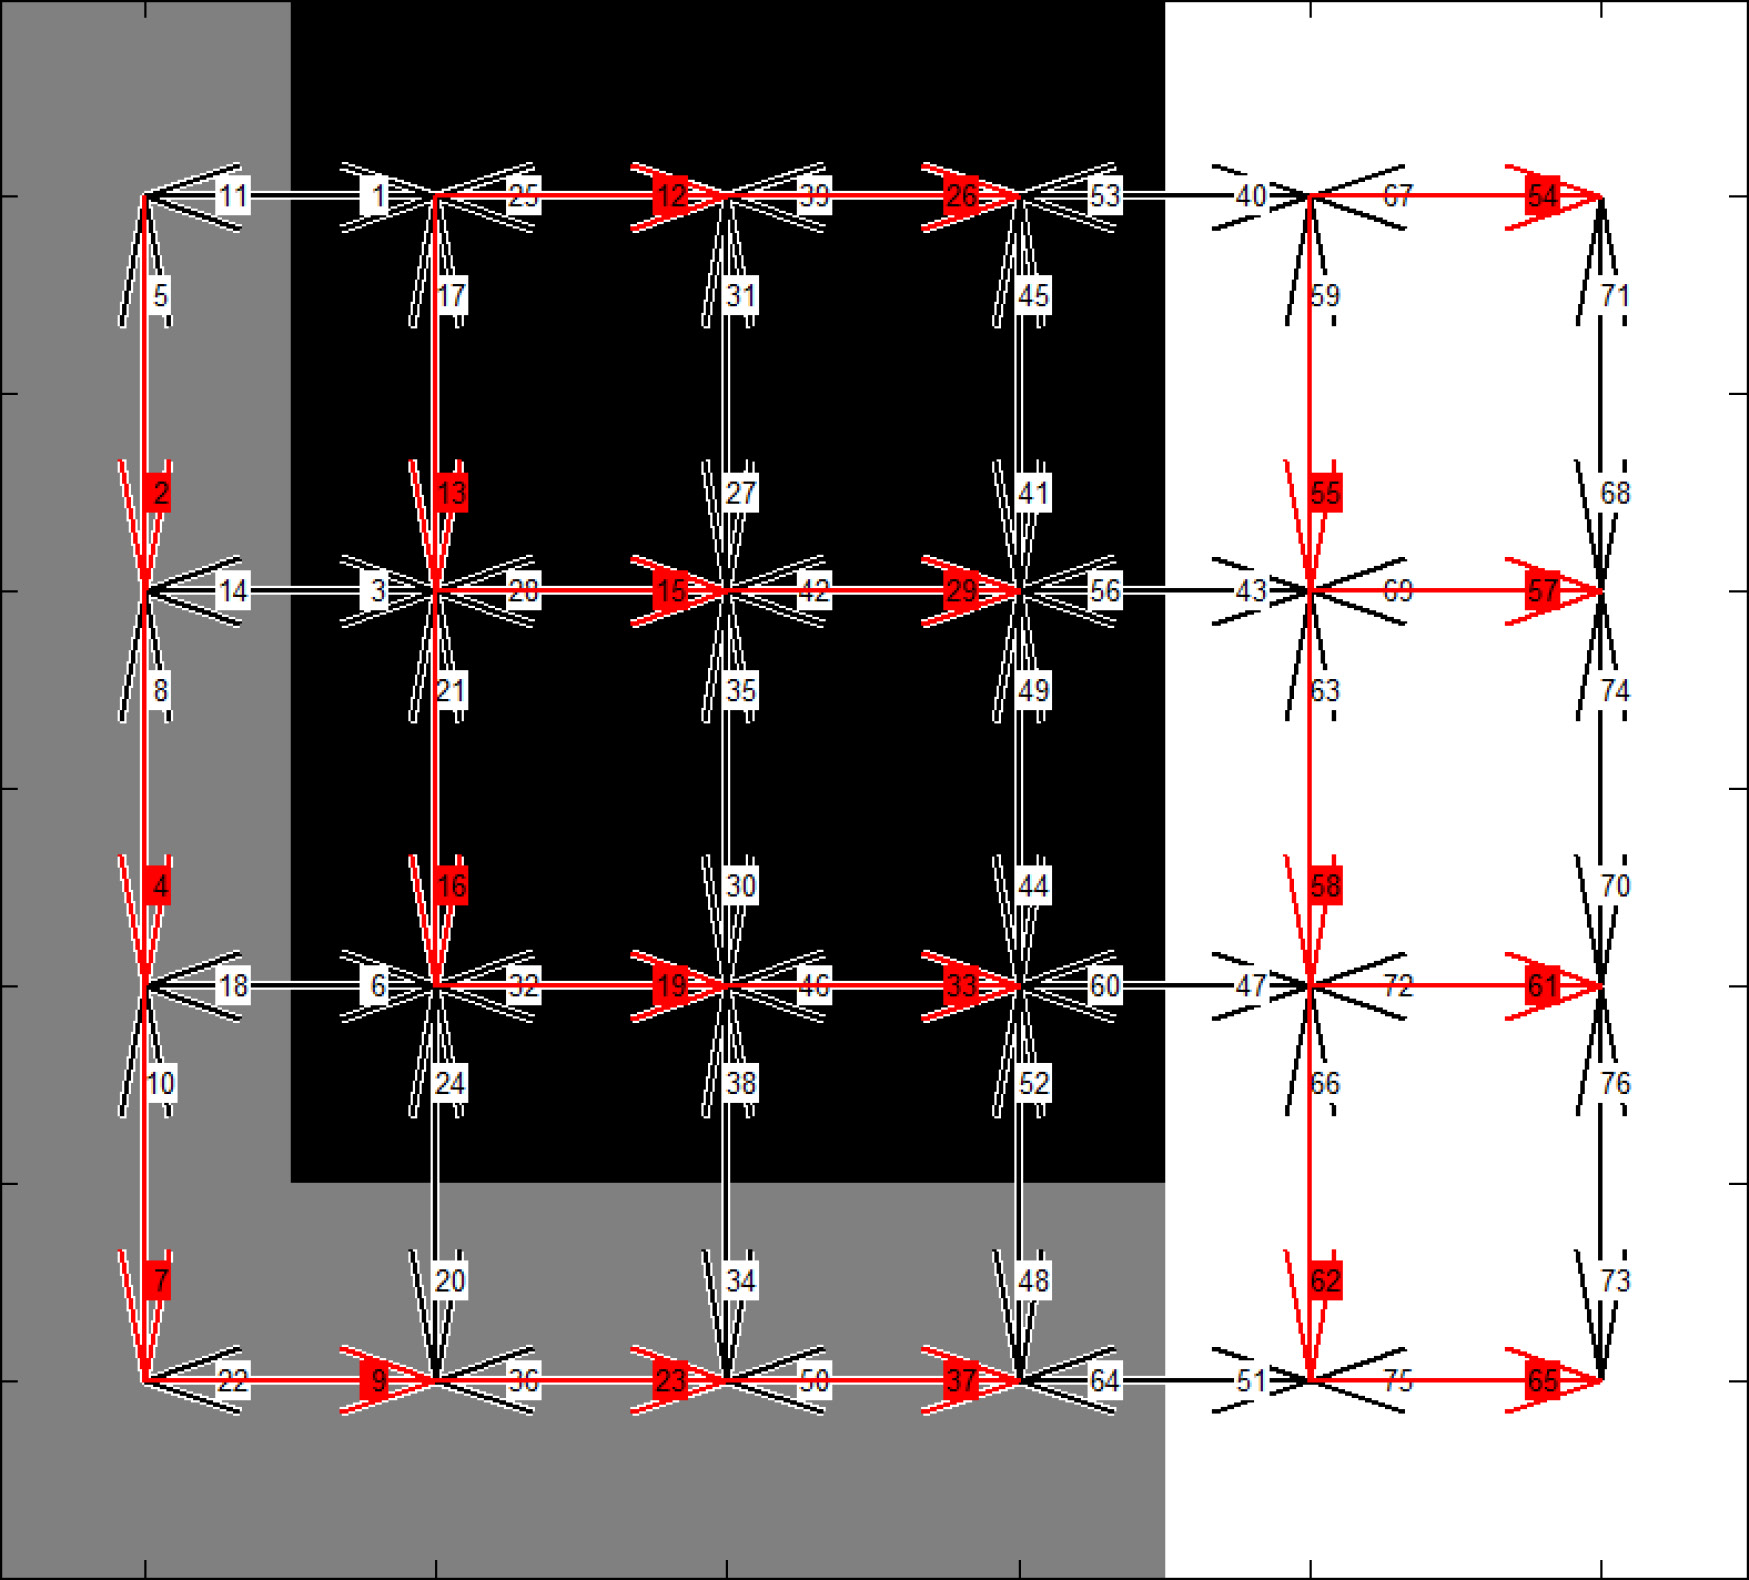
\includegraphics[width=\textwidth]{img/simply2.jpg}
      \caption{}\label{fig:dart_simply2}
    \end{subfigure}
    ~
    \begin{subfigure}[b]{0.3\textwidth}
      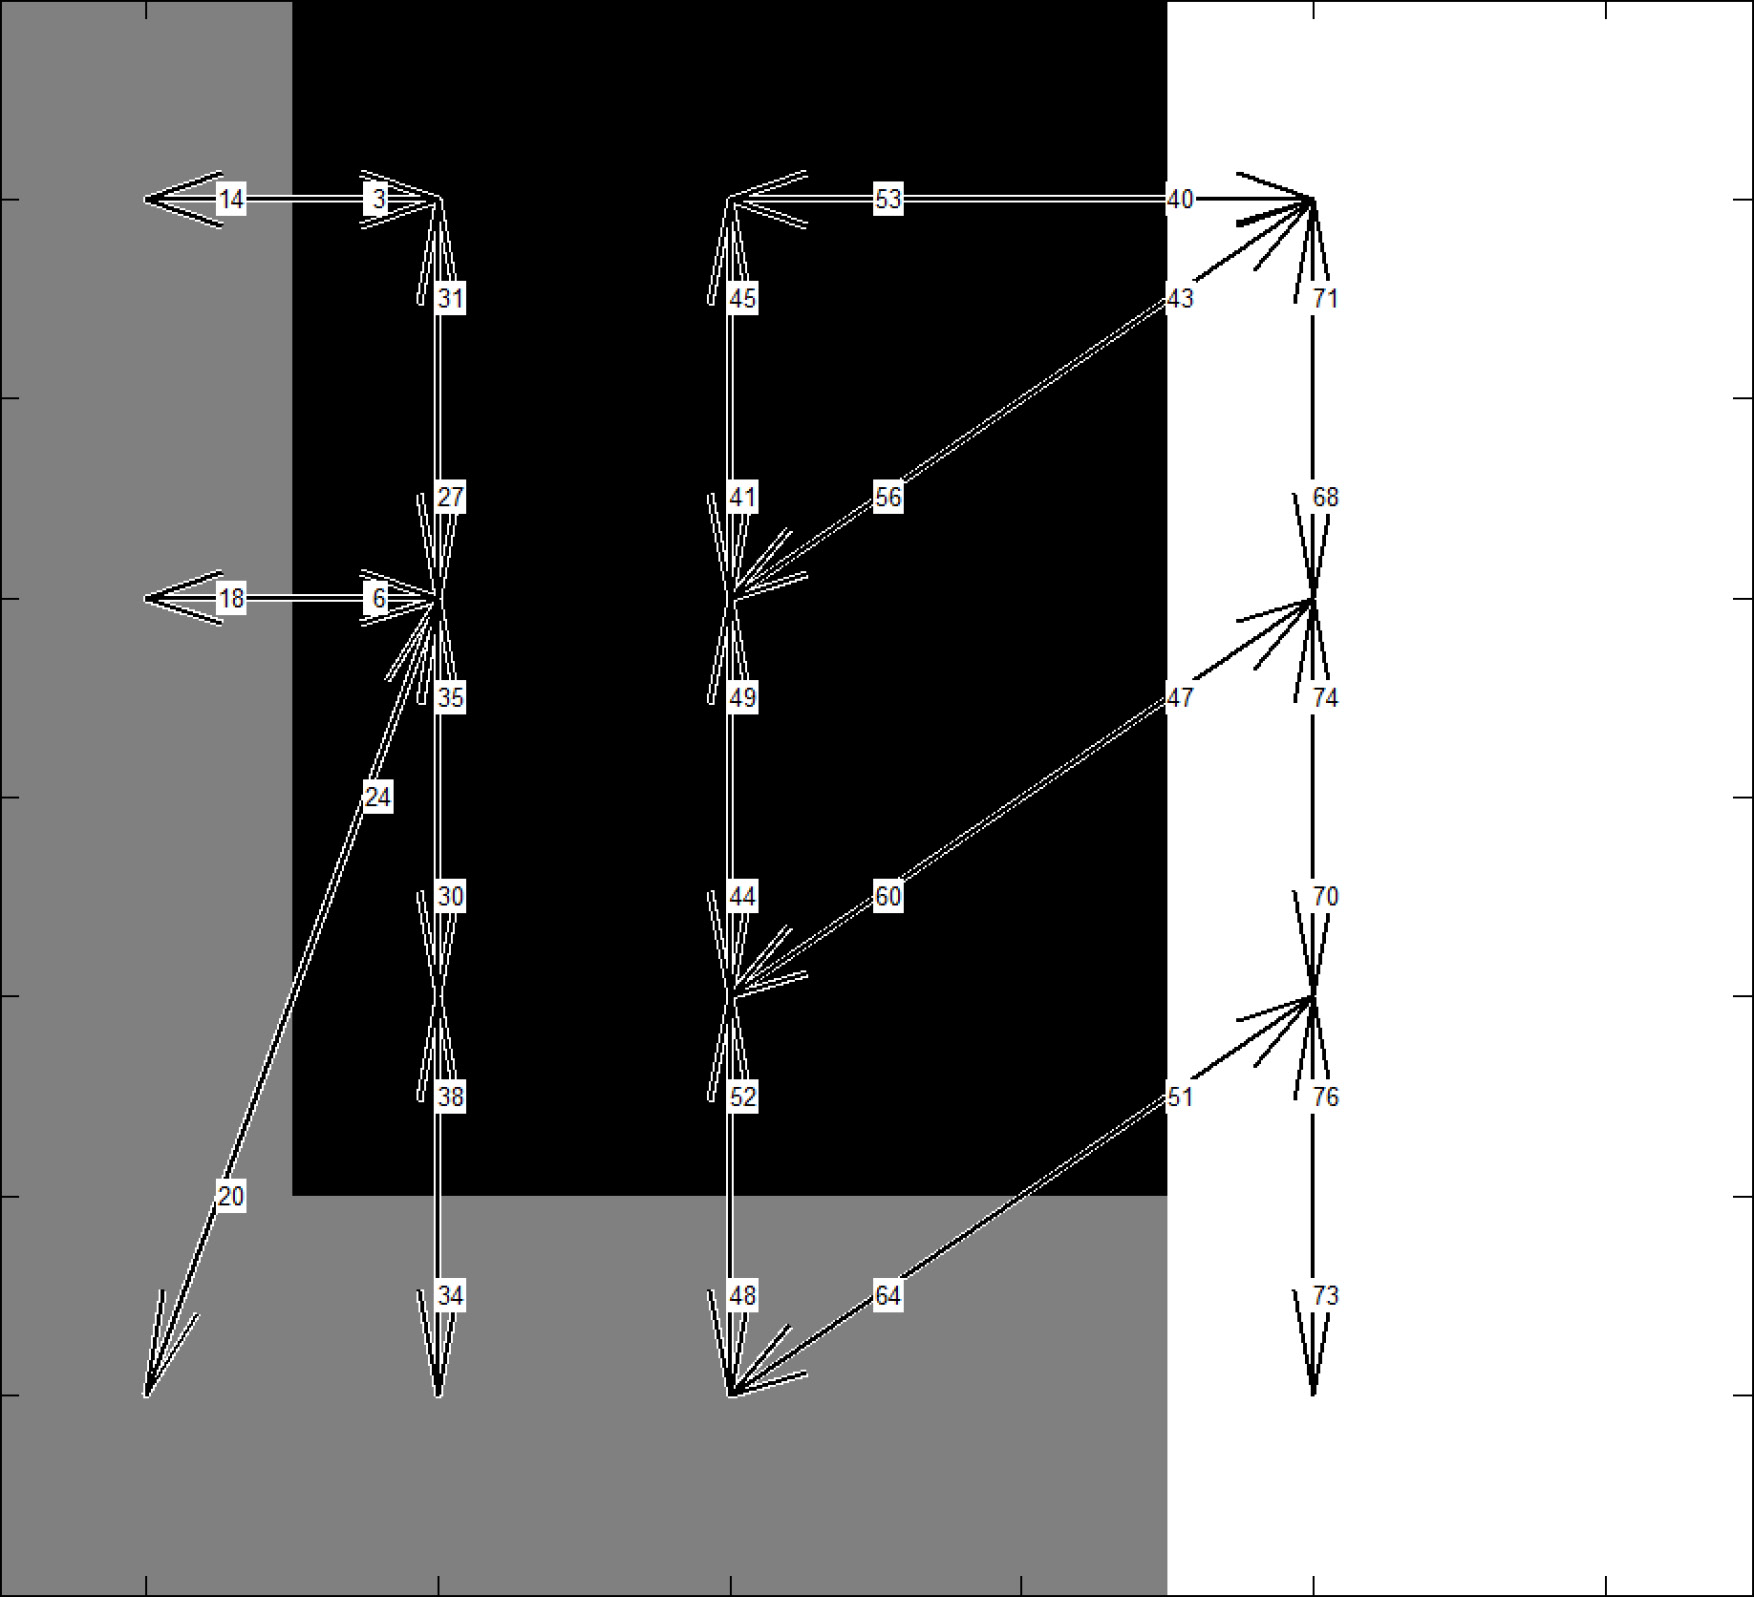
\includegraphics[width=\textwidth]{img/simply3.jpg}
      \caption{}\label{fig:dart_simply3}
    \end{subfigure}
    ~
    \begin{subfigure}[b]{0.3\textwidth}
      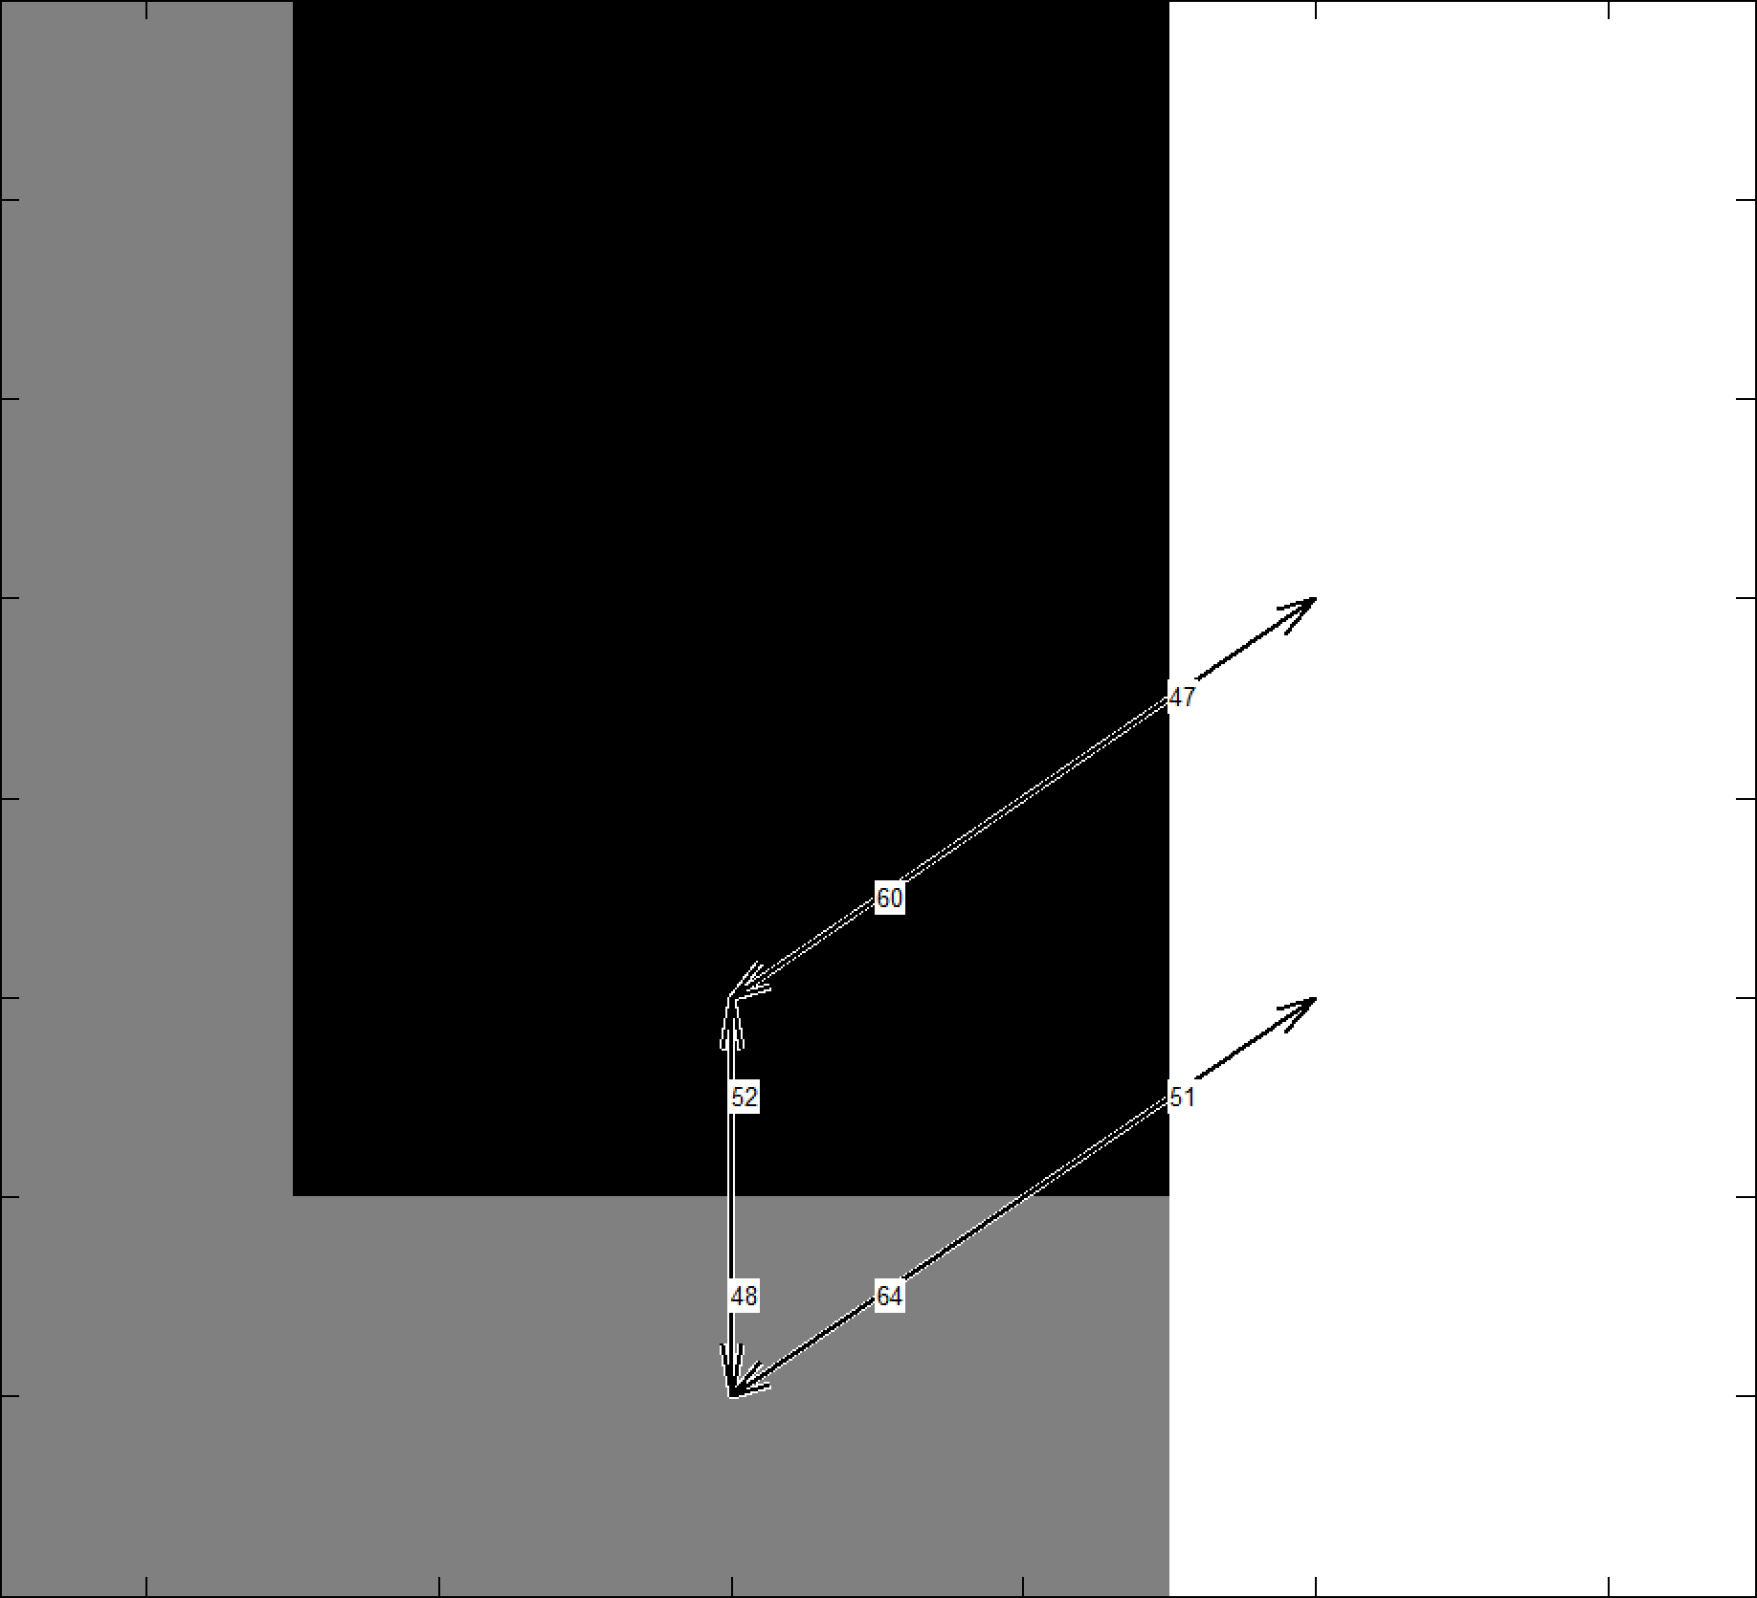
\includegraphics[width=\textwidth]{img/simply1.jpg}
      \caption{}\label{fig:dart_simply1}
    \end{subfigure}
  \caption{(a) the contraction kernel of the input image. (b) the darts after the contraction step (c) the darts after simplification}\label{fig:dart_simply}
\end{figure}

% subsection simplification (end)

% section construction_of_the_pyramid (end)

\section{Results} % (fold)
\label{sec:results}

\begin{figure}[tb]
  \centering

    \begin{subfigure}[b]{0.4\textwidth}
      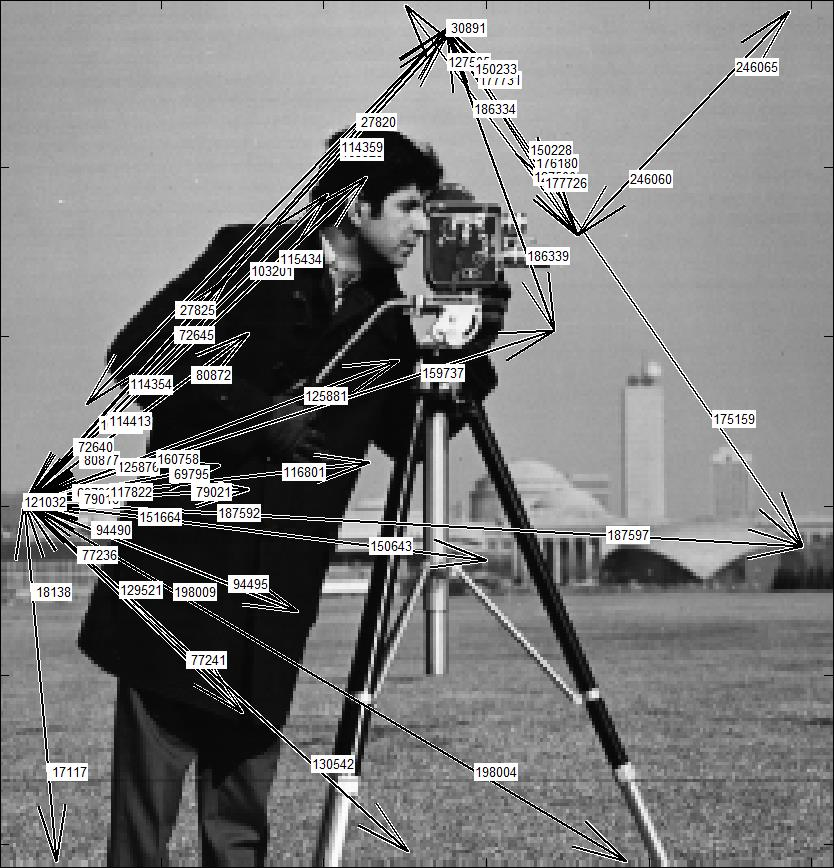
\includegraphics[width=\textwidth]{img/result.jpg}
      \caption{}\label{fig:result1}
    \end{subfigure}
    ~
    \begin{subfigure}[b]{0.4\textwidth}
      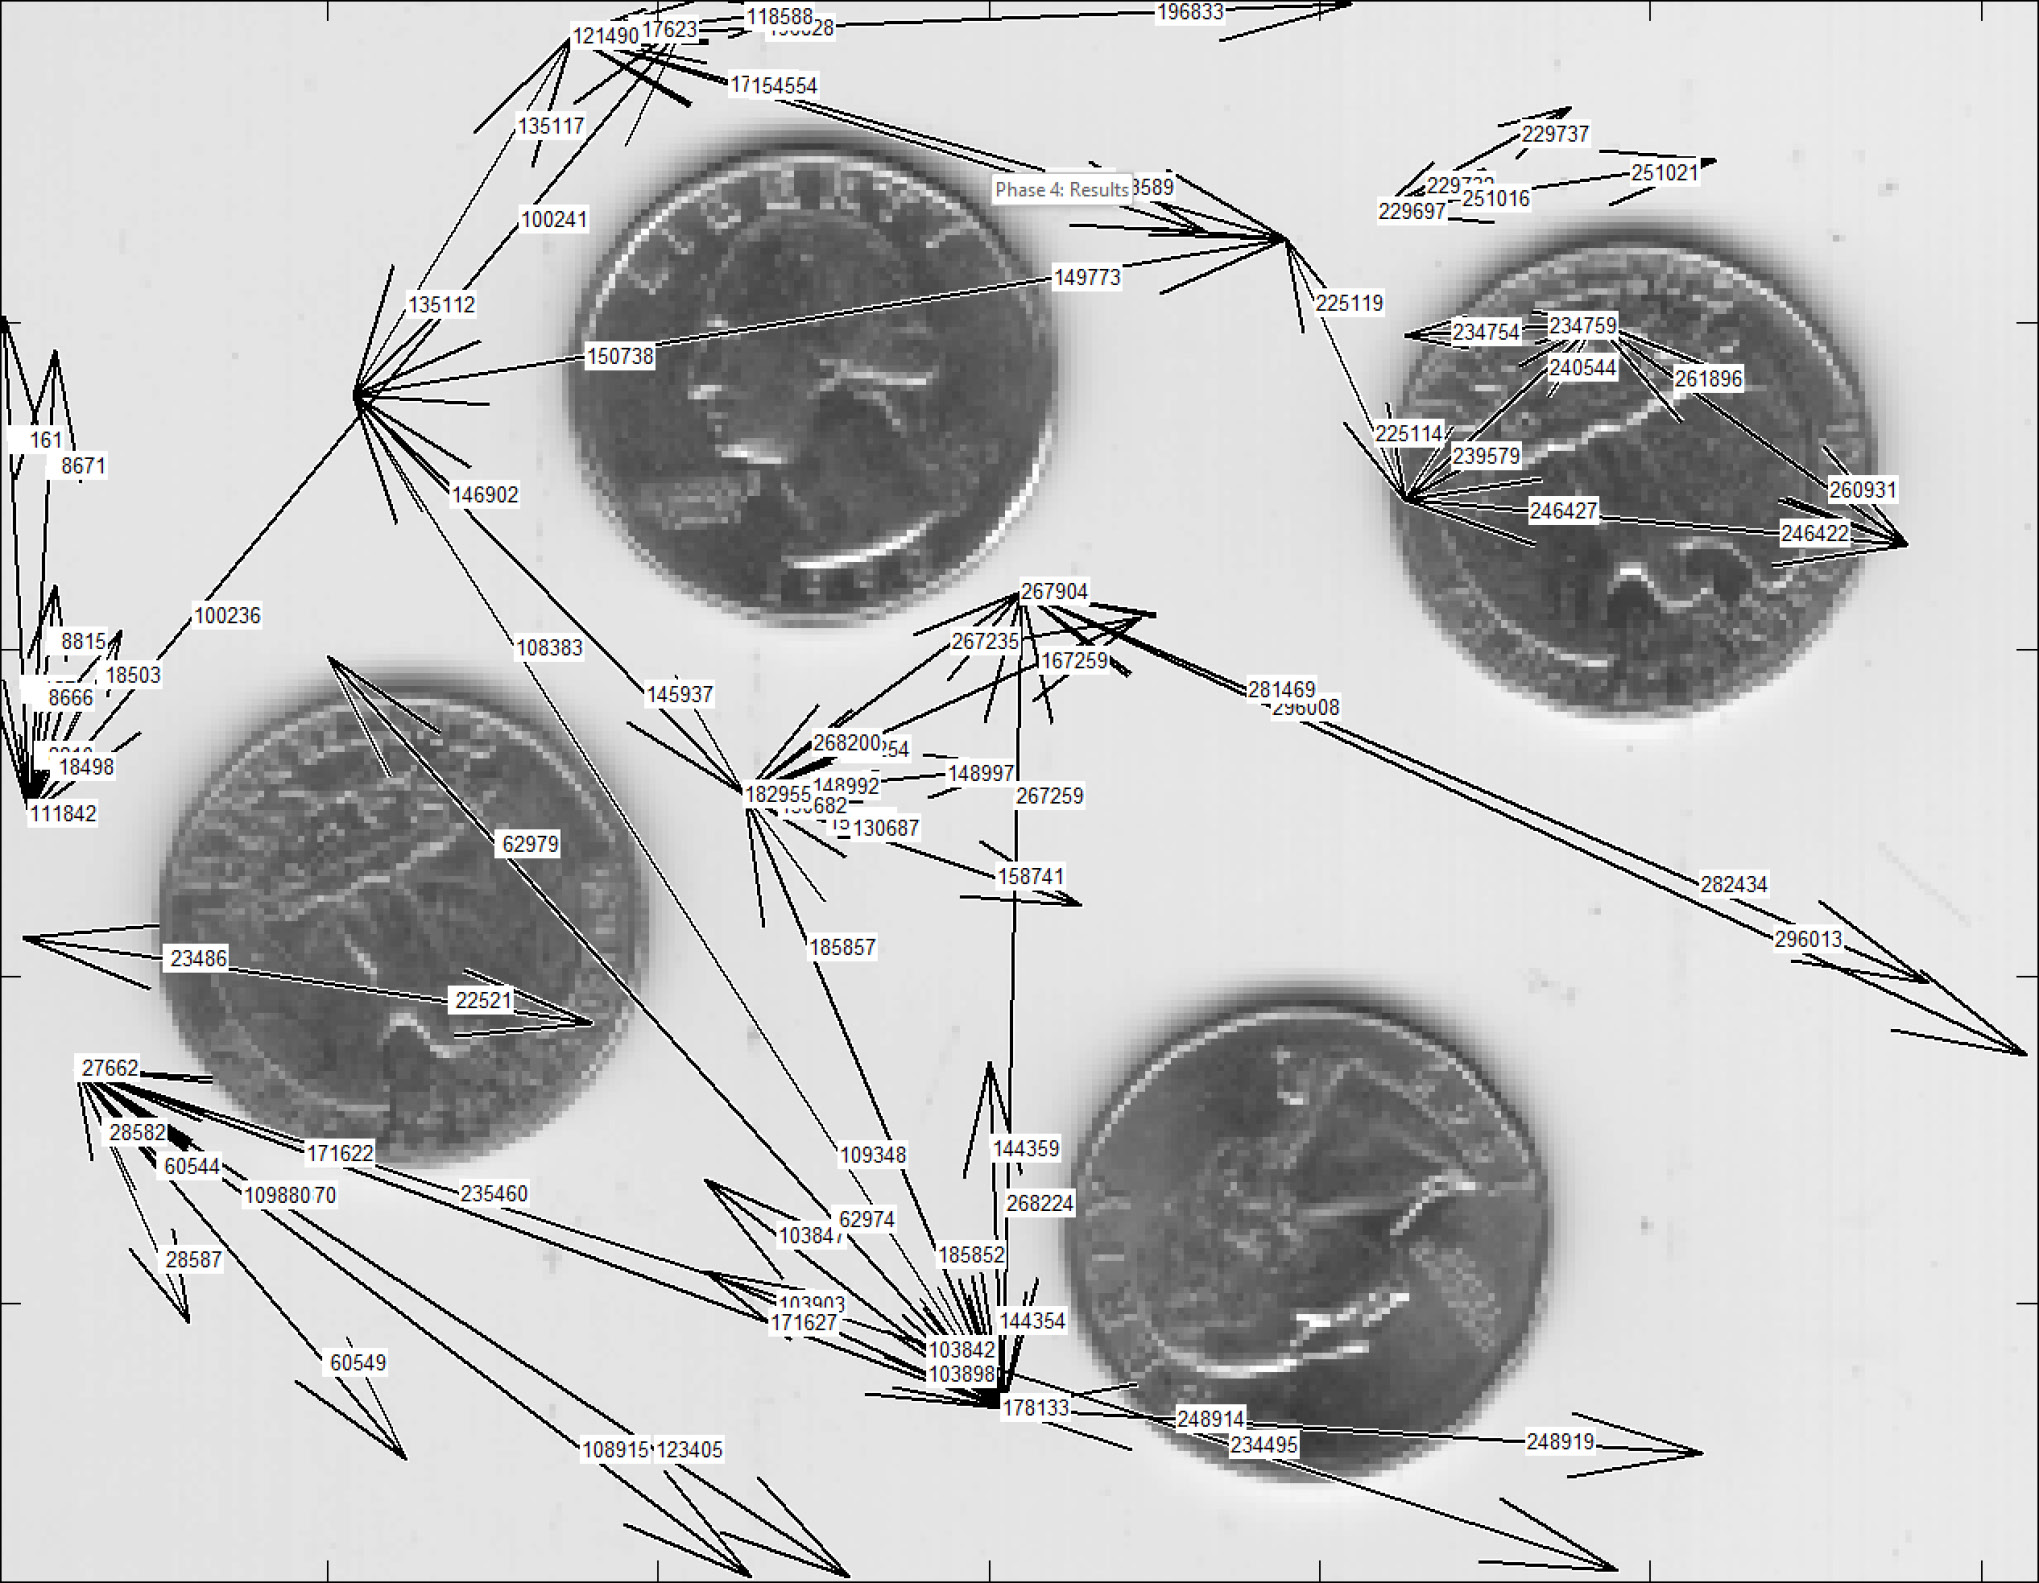
\includegraphics[width=\textwidth]{img/result2.jpg}
      \caption{}\label{fig:result2}
    \end{subfigure}
  \caption{The two test images. The shown darts are the darts of the top pyramid level.}\label{fig:result}
\end{figure}

\subsection{Performance} % (fold)
\label{sub:performance}

\begin{table}[tb]
  \caption{caption here}
  \label{tab:tablename}
  \centering

  \begin{tabular}{lcc}
  \toprule
  \textbf{Image} & \textbf{initial CM} & \textbf{Contraction\\ level 1} & \textbf{Simplification\\ level 1} & \textbf{Total}\\
    \cref{fig:result1} & 0.05 & & &\\
    \cref{fig:result2} & & & &\\
  \bottomrule
  \end{tabular}
\end{table}

The implementation was tested on a  Processor Intel(R) Core(TM) i7-3770K CPU @ 3.50GHz, 3501 Mhz, 4 Core(s), 8 Logical Processor(s) with installed 16,0 GB physical memory (RAM).

The bottle neck of the implementation was the simplification process. Which took for the two.

% subsection performance (end)

\subsection{Publication} % (fold)
\label{sub:publication}

I published my work on the platform \texttt{Github}\cite{github}. The repository is called: \url{https://github.com/theShmoo/CombiPyr-ImSeg} and it contains:
\begin{itemize}
  \item The source code of the \texttt{Python} implementation (\cref{sub:python_implementation}).
  \item The source code of the \texttt{Matlab} implemenation (\cref{sec:computation_of_the_dart_values,sec:construction_of_the_initial_cm_level,sec:construction_of_the_pyramid}).
  \item My presentation of the work, held in the lecture.
  \item This documentation.
\end{itemize}

% subsection publication (end)


% section results (end)

%-----------------------------------------------------------------------------
\bibliographystyle{abbrv}
\bibliography{bibliography}


\end{document}
